\documentclass[11pt,a4paper]{article}
\usepackage[margin=2.2cm]{geometry}
\usepackage{lmodern}
\usepackage[T1]{fontenc}
\usepackage[utf8]{inputenc}
\usepackage{amsmath,amssymb,amsthm}
\usepackage{booktabs,array,tabularx,longtable}
\usepackage{enumitem}
\usepackage{xcolor}
\usepackage[most]{tcolorbox}
\usepackage{titlesec}
\usepackage{graphicx}
\usepackage{float}
\usepackage{adjustbox}
\usepackage{tikz}
\usetikzlibrary{arrows.meta,positioning,calc,fit,backgrounds}
\usepackage[font=small,labelfont={bf,color=headblue},skip=4pt]{caption}
\usepackage[colorlinks=true,linkcolor=headblue,citecolor=headblue,urlcolor=blue!50!black]{hyperref}

\definecolor{headblue}{RGB}{38,70,120}
\definecolor{accent}{RGB}{42,120,214}
\definecolor{accent2}{RGB}{235,104,52}
\definecolor{accent3}{RGB}{27,175,122}
\titleformat{\part}[display]{\centering\Huge\bfseries\color{headblue}}{Part \thepart}{10pt}{}
\titleformat{\section}{\Large\bfseries\color{headblue}}{\thesection}{0.8em}{}[{\color{black}\titlerule}]
\titleformat{\subsection}{\large\bfseries\color{headblue}}{\thesubsection}{0.8em}{}
\titleformat{\subsubsection}{\normalsize\bfseries\color{headblue}}{\thesubsubsection}{0.8em}{}
\titlespacing*{\section}{0pt}{12pt}{6pt}
\titlespacing*{\subsection}{0pt}{9pt}{3pt}
\setlength{\parindent}{0pt}
\setlength{\parskip}{5pt}
\setlist{itemsep=1pt,topsep=2pt}
\renewcommand{\arraystretch}{1.12}
\setlength{\emergencystretch}{3em}

% ---- boxes ---------------------------------------------------------------
\newtcolorbox{keybox}{colback=blue!3,colframe=headblue!60,boxrule=0.5pt,arc=2mm,left=2mm,right=2mm,top=1mm,bottom=1mm}
\newtcolorbox{insum}{colback=green!3,colframe=green!40!black,boxrule=0.4pt,arc=1.5mm,left=2mm,right=2mm,top=0.5mm,bottom=0.5mm,fontupper=\small}
\newcommand{\inshort}[1]{\begin{insum}\textbf{In short.} #1\end{insum}}
\newtcolorbox{whybox}{colback=orange!3,colframe=orange!65!black,boxrule=0.4pt,arc=1.5mm,left=2mm,right=2mm,top=0.5mm,bottom=0.5mm,fontupper=\small}
\newcommand{\practical}[1]{\begin{whybox}\textbf{Why it happens (practical).} #1\end{whybox}}
\newtcolorbox{supportbox}{colback=headblue!4,colframe=headblue!45,boxrule=0.4pt,arc=1.5mm,left=2mm,right=2mm,top=0.5mm,bottom=0.5mm,fontupper=\small}
\newcommand{\support}[1]{\begin{supportbox}\textbf{How the result is supported.} #1\end{supportbox}}
\newcommand{\code}[1]{\texttt{#1}}
\let\origunderscore\_
\renewcommand{\_}{\origunderscore\allowbreak}

% ---- proposition / proof -------------------------------------------------
\theoremstyle{definition}
\newtheorem{proposition}{Proposition}
\newtheorem{corollary}{Corollary}
\renewcommand{\qedsymbol}{$\blacksquare$}

\newcommand{\fcomShareData}{70}
\newcommand{\fthetaPersData}{0.69}
\newcommand{\fthetaComData}{0.36}
\newcommand{\fstrandedData}{15}
\newcommand{\fpF}{15}
\newcommand{\fpM}{25}
\newcommand{\fmilpOptimal}{277}
\newcommand{\fmilpTL}{197}
\newcommand{\fmilpTLnoPlan}{35}
\newcommand{\fmilpInfeasible}{51}
\newcommand{\fmilpValid}{474}
\newcommand{\fmilpGapMedian}{3.3}
\newcommand{\fmilpGapMean}{5.7}
\newcommand{\fmilpSolveMean}{140}
\newcommand{\fgreedyValid}{461}
\newcommand{\fshareZOne}{0.9}
\newcommand{\fshareZTwo}{2.4}
\newcommand{\fshareZThree}{7.5}
\newcommand{\fshareZFour}{20.9}
\newcommand{\fshareZFive}{39.3}
\newcommand{\fshareZSix}{29.0}
\newcommand{\fshareOperator}{30.8}
\newcommand{\fmilpMeanZ}{43,999}
\newcommand{\frlValid}{500}
\newcommand{\frlInvalid}{60}
\newcommand{\frlPaired}{474}
\newcommand{\frlGapMean}{0.85}
\newcommand{\frlGapMedian}{0.76}
\newcommand{\frlGapOpt}{0.92}
\newcommand{\frlOnly}{26}
\newcommand{\fmilpOnly}{0}
\newcommand{\frlBetter}{28}
\newcommand{\frlSolveMean}{0.12}
\newcommand{\frlOnlyFromNoPlan}{26}
\newcommand{\frlOnlyFromInfeasible}{0}
\newcommand{\frlParams}{765,858}
\newcommand{\frlTrainMin}{39}
\newcommand{\frlBestEpoch}{180}
\newcommand{\frlStopEpoch}{210}
\newcommand{\frlBestVal}{0.969}
\newcommand{\frlUntrained}{3.57}
\newcommand{\frlAfterWarmOne}{1.167}
\newcommand{\fvanPersMilp}{19.9}
\newcommand{\fvanComMilp}{0.7}
\newcommand{\fvanPersRl}{6.7}
\newcommand{\fvanComRl}{0.9}
\newcommand{\fqueueComMilp}{1.58}
\newcommand{\fqueuePersMilp}{0.41}
\newcommand{\fthetaStarPers}{0.95}
\newcommand{\fagreeZsMean}{0.14}
\newcommand{\fagreeRtMean}{0.16}
\newcommand{\fagreeSign}{13}
\newcommand{\fnVariants}{15}
\newcommand{\fdZEvcCipersonalviipv}{-2.21}
\newcommand{\fdZEvcCipersonaliiipv}{+2.08}
\newcommand{\fdZEvomegaicommercialivpv}{-2.67}
\newcommand{\fdZEvomegaicommercialviipv}{+2.66}
\newcommand{\fdZEvimuopersonalipiiiv}{-1.35}
\newcommand{\fdZEvimuopersonalipviiiviiv}{+1.33}
\newcommand{\fdZEvimuocommercialipiiiv}{-6.38}
\newcommand{\fdZEvimuocommercialipviiiviiv}{+6.43}
\newcommand{\fdZEipMiv}{-4.19}
\newcommand{\fdZEipMiiiv}{+3.91}
\newcommand{\fdZEiivansiii}{-0.04}
\newcommand{\fdZEiivansvii}{+0.02}
\newcommand{\fdZEiiseatsiv}{+1.08}
\newcommand{\fdZEiiseatsviii}{-0.08}
\newcommand{\fdZEviiibatteryiioo}{-0.01}
\newcommand{\fdirectionBad}{0}
\newcommand{\feNineGunsHalfDz}{+4.8}
\newcommand{\feNineGunsHalfLost}{68}
\newcommand{\feNineGunsHalfGain}{0}
\newcommand{\feNineGunsDblDz}{-2.2}
\newcommand{\feNineGunsDblLost}{0}
\newcommand{\feNineGunsDblGain}{9}
\newcommand{\feNinePowHalfDz}{+20.1}
\newcommand{\feNinePowHalfLost}{102}
\newcommand{\feNinePowHalfGain}{0}
\newcommand{\feNinePowDblDz}{-12.3}
\newcommand{\feNinePowDblLost}{0}
\newcommand{\feNinePowDblGain}{32}
\newcommand{\fmeanEnergy}{19}
\newcommand{\feNineTauHalf}{106}
\newcommand{\feNineTauBase}{53}
\newcommand{\feNineTauDbl}{27}
\newcommand{\feNinePowDblDzAbs}{12.3}
\newcommand{\feNineGunsDblDzAbs}{2.2}
\newcommand{\feNinePowHalfVan}{59}
\newcommand{\feNineGunsHalfQ}{3.5}
\newcommand{\feNineGunsHalfQBase}{1.2}
\newcommand{\feTenDownDz}{-21.8}
\newcommand{\feTenUpDz}{+22.2}
\newcommand{\feTenSlope}{88}
\newcommand{\feTenElastic}{0.88}
\newcommand{\feTenUpLost}{79}
\newcommand{\feTenDownGain}{39}
\newcommand{\feTenDownDzAbs}{21.8}
\newcommand{\feTenNonElastic}{12}


\hypersetup{pdftitle={Formulation 4: a results analysis report}, pdfauthor={Yakshith Maddineni}}

\begin{document}

\begin{titlepage}
\centering
\vspace*{1.6cm}
{\LARGE\bfseries\color{headblue} EV Charging Network Optimisation\par}
\vspace{8pt}
{\Large\bfseries Formulation 4 --- a results analysis report\par}
\vspace{6pt}
{\large Theory, practice and evidence for every experiment\par}
\vspace{10pt}
{\large MILP (Gurobi) and reinforcement learning, two customer segments\par}
\vspace{22pt}
{\large CP 320 --- Operations Research for Mobility Management\par}
{\normalsize Course project\par}
\vspace{20pt}
{\large Yakshith Maddineni \quad (SR 26080)\par}
{\normalsize M.Tech Smart Mobility \& Logistics Systems, IISc\par}
\vspace{6pt}
{\normalsize \today\par}
\vfill
\begin{keybox}
\textbf{What this report is.} A self-contained analysis of the results of formulation~4 of the EV charging
network problem. For the baseline and for \emph{every} experiment it gives four things, in this order:
(i)~the \textbf{mathematical/theoretical} prediction derived from the model itself; (ii)~the \textbf{empirical
result} as figures and tables; (iii)~the \textbf{practical} reason the result comes out that way; and
(iv)~\textbf{how the result is supported} --- by a direction check that the optimiser must obey, by the
agreement of the two independent methods, and by internal consistency.

\textbf{The two methods.} The problem is solved exactly by a Gurobi MILP and approximately by a reinforcement-learning
policy; every plan from either method is scored by the same independent checker of constraints (2)--(23) and
objective~\eqref{eq:obj}, so their costs are directly comparable.

\textbf{Scope.} Baseline $+$ seven experiments $=$ E1 (van tariff), E2 (mobile-charger fleet and seats),
E5 (value of charging time), E6 (money sensitivity), E8 (van battery), E9 (station capacity: guns and power),
E10 (charging demand). E1--E8 were solved by both methods; E9--E10 by the RL policy, retrained per setting.
\end{keybox}
\end{titlepage}

\tableofcontents
\newpage

\part{The problem and the optimisation model}
%=====================================================================
\section{The problem}
\label{sec:intro}

An operator must charge a set of electric vehicles (EVs) during one planning period. Each EV sends a
\emph{request} at a known time and needs a known amount of energy. The operator has two kinds of resource:
\begin{itemize}
  \item \textbf{Fixed charging stations (FCS)} with a few \emph{guns} each; an EV drives to a station, may
  \emph{queue} for a free gun, then charges at the gun's power;
  \item \textbf{Mobile charging stations (MCS)} --- a fleet of \emph{vans} that drive out from a depot, visit
  EVs where they are parked, and charge them on the spot at a higher power. A van serves several EVs on a route
  and is limited by its seats (how many EVs it can serve), its battery and the length of the period.
\end{itemize}
The operator decides, for every EV, whether it charges at a station or is served by a van, and it routes and
schedules the vans, so as to \textbf{serve every request before the deadline} at the \textbf{least total cost}.

\subsection{Two kinds of customer (what formulation 4 adds)}

Formulation~4 keeps the variables and all constraints (1)--(23) of formulation~3 and adds one fact about every
EV: its \textbf{use segment} $s_i\in\{\mathrm P,\mathrm C\}$ --- \emph{personal} (a private car) or
\emph{commercial} (a taxi, ride-hailing or fleet car) --- together with an \textbf{income index}
$\theta_i\in[0,1]$. These two attributes change how a customer values money and time:
\begin{itemize}
  \item a \textbf{personal} driver's time depends on \emph{where} the driver is: driving, queueing and charging
  \emph{at a station} cost the driver's time, but when a \emph{van} charges the parked car the driver is free,
  so those minutes are cheaper;
  \item a \textbf{commercial} car earns nothing while out of service: every minute of driving, queueing,
  charging or waiting for a van costs the same lost earnings (the \emph{downtime} rate). A van gives a taxi no
  ``driver-free'' benefit; it only saves downtime.
\end{itemize}
This single distinction is what makes the results interesting: the \emph{same} plan is good or bad for a
customer depending on whether the car is a private car or a taxi, and on how rich the household is.

\subsection{What ``cost'' means here}

The operator minimises its own running cost \emph{plus} the cost its customers \emph{perceive}. A customer's
perceived cost is the money they pay times how strongly they feel a rupee, plus the value of the time they lose.
Tariff income is a transfer (the customer pays, the operator receives), so it is not counted as an operator
gain; it enters only through what the customer feels. Section~\ref{sec:model} writes this as the six-part
objective $Z=Z_1+\dots+Z_6$.

\subsection{How this report reads}

Every result below --- the baseline and each of the seven experiments --- is presented in the same four steps,
so the reasoning is always visible:
\begin{enumerate}
  \item \textbf{Theory.} What the model \emph{must} do, derived from the objective~\eqref{eq:obj} or a
  constraint, stated as a short proposition with a proof.
  \item \textbf{Result.} What actually happened, as a figure and a table of the measured numbers.
  \item \textbf{Practical cause.} Why the plan comes out that way, in plain operational terms.
  \item \textbf{Support.} Why the number can be trusted: a direction the optimiser cannot violate, the
  agreement of the MILP and the RL policy (two independent methods), and internal consistency.
\end{enumerate}

\inshort{Assign every EV to a station or a van and route the vans, at least total cost, serving all requests
before the deadline. Formulation~4 adds a segment (personal / commercial) and an income to every customer,
which changes how each values money and time. This report explains every result by theory, evidence, practical
cause and independent support.}

%=====================================================================
\section{The optimisation model}
\label{sec:model}

The problem is a mixed-integer linear program (MILP). Figure~\ref{fig:schematic} shows the picture; this section
writes the objective and the constraints that the experiments act on, and derives the one piece of theory that
every later result rests on: when the model prefers a van to a station.

\begin{figure}[H]
\centering
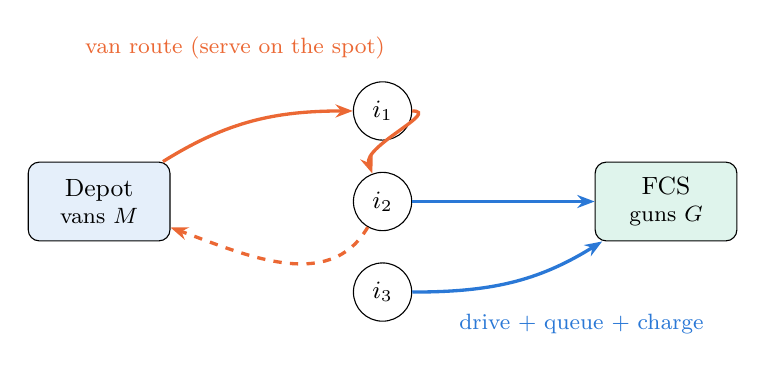
\begin{tikzpicture}[font=\small,>={Stealth[length=2.2mm]},
  box/.style={draw,rounded corners,align=center,minimum height=1.0cm,minimum width=1.8cm},
  ev/.style={circle,draw,fill=white,minimum size=0.74cm,inner sep=1pt}]
  \node[box,fill=accent!12] (depot) at (0,0) {Depot\\[-1pt]{\footnotesize vans $M$}};
  \node[ev] (e1) at (3.6,1.15) {$i_1$};
  \node[ev] (e2) at (3.6,0) {$i_2$};
  \node[ev] (e3) at (3.6,-1.15) {$i_3$};
  \node[box,fill=accent3!14] (fcs) at (7.2,0) {FCS\\[-1pt]{\footnotesize guns $G$}};
  \draw[->,accent2,very thick] (depot) to[out=32,in=180] (e1);
  \draw[->,accent2,very thick] (e1) to[out=0,in=110] (e2);
  \draw[->,accent2,very thick,dashed] (e2) to[out=-120,in=-20] (depot);
  \draw[->,accent,very thick] (e2) -- (fcs);
  \draw[->,accent,very thick] (e3) to[out=0,in=212] (fcs);
  \node[font=\footnotesize,text=accent2,anchor=west] at (-0.3,1.95) {van route (serve on the spot)};
  \node[font=\footnotesize,text=accent,anchor=west] at (4.45,-1.55) {drive $+$ queue $+$ charge};
\end{tikzpicture}
\caption{Each EV $i$ is served by \emph{one} resource: it drives to a fixed station and queues for a gun
(blue), or a van visits it on a route from the depot and charges it in place (orange). The model chooses the
assignment, routes the vans and schedules all charging in continuous time.}
\label{fig:schematic}
\end{figure}

\subsection{Decision variables}
For every EV $i$: a binary $y_{ig}$ (charge at gun $g$) and $z_{im}$ (served by van $m$); the route variables
$x_{ijm}$ (van $m$ goes $i\!\to\!j$) and $u_m$ (van $m$ is used); and continuous times $S_i$ (start of charging),
$q^{\mathrm F}_i$ (queue at the station) and $q^{\mathrm M}_i$ (wait for the van). Write
$y_i=\sum_g y_{ig}$, $z_i=\sum_m z_{im}$ (so $y_i+z_i=1$), and the completion time
$C_i=S_i+\tau^{\mathrm F}_iy_i+\tau^{\mathrm M}_iz_i$. Charging \emph{durations} are fixed by the physics
\begin{equation}
\tau^{\mathrm F}_i=\frac{60\,E_i}{P^{\mathrm F}},\qquad \tau^{\mathrm M}_i=\frac{60\,E_i}{P^{\mathrm M}}
\quad\text{(minutes)},\qquad P^{\mathrm M}>P^{\mathrm F},
\label{eq:tau}
\end{equation}
with $E_i$ the energy demand (kWh) and $P^{\mathrm F},P^{\mathrm M}$ the FCS and van powers (kW).

\subsection{The objective}
\begin{equation}
\begin{aligned}
\min\ Z \;=\;& \underbrace{\sum_{i}\mu_i\,c^{\mathrm{EV}}\!\sum_{f}d_{if}Y_{if}}_{Z_1:\ \text{EV driving (felt)}}
+\underbrace{c^{\mathrm M}\!\sum_{m}\sum_{(i,j)}d_{ij}x_{ijm}}_{Z_2:\ \text{van driving}}
+\underbrace{\sum_{m}c^{\mathrm F}_mu_m}_{Z_3:\ \text{van dispatch}}
+\underbrace{\pi^{\mathrm F}\!\sum_{i}E_iy_i+\pi^{\mathrm M}\!\sum_{i}\tfrac{E_i}{\eta}z_i}_{Z_4:\ \text{operator energy}}\\[2pt]
&+\underbrace{\sum_{i}\mu_i\,E_i\big(p^{\mathrm F}y_i+p^{\mathrm M}z_i\big)}_{Z_5:\ \text{tariff (felt)}}
+\underbrace{\sum_{i}\Big(c^{\mathrm D}_i\!\sum_{f}t_{if}Y_{if}+c^{\mathrm Q}_i q^{\mathrm F}_i+c^{\mathrm C}_i\tau^{\mathrm F}_iy_i+c^{\mathrm V}_i\big(q^{\mathrm M}_i+\tau^{\mathrm M}_iz_i\big)\Big)}_{Z_6:\ \text{time (felt)}}
\end{aligned}
\label{eq:obj}
\end{equation}
The operator's running cost is $Z_2+Z_3+Z_4$ (van driving, van dispatch, electricity); the customer's
\emph{perceived} cost is $Z_1+Z_5+Z_6$ (felt money for driving and tariff, and the value of lost time).
$\mu_i$ is money sensitivity and $c^{a}_i$ the value of a minute in activity $a\in\{\mathrm D,\mathrm Q,\mathrm C,\mathrm V\}$
(drive, queue, charge at FCS, van). Figure~\ref{fig:ztree} groups the six terms.

\begin{figure}[H]
\centering
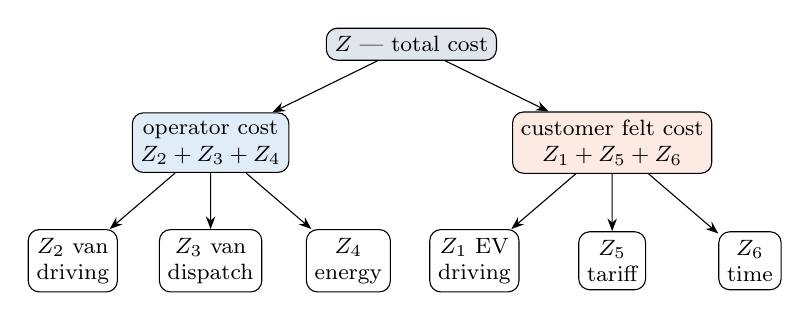
\begin{tikzpicture}[font=\footnotesize, every node/.style={rounded corners,draw,align=center,inner sep=3pt},
  level 1/.style={sibling distance=5.1cm,level distance=1.25cm},
  level 2/.style={sibling distance=1.75cm,level distance=1.5cm},
  edge from parent/.style={draw,-{Stealth[length=1.6mm]}}]
\node[fill=headblue!14]{$Z$ --- total cost}
  child {node[fill=accent!14]{operator cost\\ $Z_2+Z_3+Z_4$}
    child {node{$Z_2$ van\\ driving}}
    child {node{$Z_3$ van\\ dispatch}}
    child {node{$Z_4$\\ energy}}}
  child {node[fill=accent2!14]{customer felt cost\\ $Z_1+Z_5+Z_6$}
    child {node{$Z_1$ EV\\ driving}}
    child {node{$Z_5$\\ tariff}}
    child {node{$Z_6$\\ time}}};
\end{tikzpicture}
\caption{The objective splits into what the operator pays and what the customers feel. Most of $Z$ sits on the
customer side (tariff $Z_5$ and time $Z_6$); the experiments act on the coefficients that weight these terms.}
\label{fig:ztree}
\end{figure}

\subsection{The customer model}
Each EV carries a segment $s_i\in\{\mathrm P,\mathrm C\}$ (personal / commercial) and an income $\theta_i\in[0,1]$,
both \emph{data}. Every coefficient is a straight line in income, with its own end points per segment:
\begin{equation}
\mu^{s}(\theta)=\mu^{s,0}+(\mu^{s,1}-\mu^{s,0})\theta,\qquad
c^{a,s}(\theta)=c^{a,s,0}+(c^{a,s,1}-c^{a,s,0})\theta,\qquad
W^{s}(\theta)=W^{s,0}+(W^{s,1}-W^{s,0})\theta.
\label{eq:lines}
\end{equation}
Richer customers feel money less ($\mu$ down with $\theta$) and time more ($c^a$ up). The two segments differ in
\emph{how} time is valued:
\begin{itemize}
  \item \textbf{Personal}: driving, queueing and station-charging cost the driver's time, but van minutes are
  cheaper because the driver is free: $c^{\mathrm V,\mathrm P}\le c^{\mathrm C,\mathrm P}$, and queueing is the
  worst, $c^{\mathrm Q,\mathrm P}>c^{\mathrm D,\mathrm P}$.
  \item \textbf{Commercial}: one downtime rate prices \emph{all} out-of-service time,
  $\omega(\theta)=c^{\mathrm D,\mathrm C}=c^{\mathrm C,\mathrm C}=c^{\mathrm V,\mathrm C}$, with a queue a little
  worse, $c^{\mathrm Q,\mathrm C}=\omega+\delta$. A van gives a taxi \emph{no} driver-free discount.
\end{itemize}
Because $(s_i,\theta_i)$ are fixed before solving, $\mu_i,c^a_i,W_i$ are numbers and the model stays a linear
MILP.

\subsection{The constraints the experiments act on}
Each EV is served exactly once, $y_i+z_i=1$. The two capacity sides and the deadline are what later variants
tighten or relax:
\begin{align}
q^{\mathrm F}_i &\le W_i\,y_i, & &\text{(queue tolerance: an FCS user waits at most $W_i$)} \label{eq:qtol}\\
C_i &\le T, & &\text{(hard deadline: every car is charged by $T$)} \label{eq:deadline}\\
\textstyle\sum_{i}\tau^{\mathrm F}_i\,y_{ig} &\le T-\min_{i:g\in G_i}(r_i+t_{if(g)}), & &\text{(gun load: a gun's charging fits its window)} \label{eq:gunload}\\
\textstyle\sum_{i} z_{im} &\le Q_m\,u_m, & &\text{(van seats: at most $Q_m$ EVs per van)} \label{eq:vancap}\\
\textstyle\sum_{i}\tfrac{E_i}{\eta}z_{im}+\beta\!\sum_{(i,j)}d_{ij}x_{ijm} &\le B_m\,u_m, & &\text{(van battery: energy served $+$ driving $\le B_m$)} \label{eq:vanbatt}
\end{align}
plus station sequencing (no two EVs on a gun at once), van routing (each van leaves and returns once), and the
number of guns per station $|G_f|$ and vans $|M|$. The experiments change exactly one of these numbers at a time:
$p^{\mathrm M}$ in $Z_5$ (E1); $|M|$ and $Q_m$ in \eqref{eq:vancap} (E2); $c^{\mathrm C,\mathrm P}$ and $\omega$ in
$Z_6$ (E5); $\mu$ in $Z_1,Z_5$ (E6); $B_m$ in \eqref{eq:vanbatt} (E8); $|G_f|$ and $P^{\mathrm F}$ in
\eqref{eq:gunload}, \eqref{eq:tau} (E9); $E_i$ everywhere it appears (E10).

\subsection{The core theory: when a van beats a station}
\label{sec:theory}
Fix the rest of the plan and compare, for EV $i$, charging at a station (queue $q^{\mathrm F}_i$) against a van
(wait $q^{\mathrm M}_i$). Let $\Pi_i=(p^{\mathrm M}-p^{\mathrm F})E_i-c^{\mathrm{EV}}d_{if}$ be the extra money the
van costs the \emph{customer} and $\kappa_i=(\pi^{\mathrm M}/\eta-\pi^{\mathrm F})E_i+c^{\mathrm M}(\text{extra van km})$
the extra cost to the \emph{operator} (neither depends on the customer's taste). The change in $Z$ from moving $i$
to a van is $\Delta_i$; the van is preferred when $\Delta_i<0$:
\begin{align}
\Delta^{\mathrm P}_i(\theta)&=\mu^{\mathrm P}(\theta)\,\Pi_i+\kappa_i
-\Big[c^{\mathrm D,\mathrm P}t_{if}+c^{\mathrm Q,\mathrm P}q^{\mathrm F}_i+c^{\mathrm C,\mathrm P}\tau^{\mathrm F}_i
-c^{\mathrm V,\mathrm P}\big(q^{\mathrm M}_i+\tau^{\mathrm M}_i\big)\Big] &&\text{(personal)},\label{eq:delP}\\
\Delta^{\mathrm C}_i(\theta)&=\mu^{\mathrm C}(\theta)\,\Pi_i+\kappa_i-\omega(\theta)\,D_i-\delta(\theta)\,q^{\mathrm F}_i,
\quad D_i=t_{if}+q^{\mathrm F}_i+\tau^{\mathrm F}_i-\big(q^{\mathrm M}_i+\tau^{\mathrm M}_i\big) &&\text{(commercial)}.\label{eq:delC}
\end{align}
$D_i$ is the downtime the van saves. Three facts follow and recur throughout the results:

\begin{keybox}
\textbf{(T1) The driver-free benefit belongs to personal cars.} In the same situation with equal money
sensitivity, $\Delta^{\mathrm C}_i-\Delta^{\mathrm P}_i=(\mu^{\mathrm C}-\mu^{\mathrm P})\Pi_i
+(\omega-c^{\mathrm V,\mathrm P})(q^{\mathrm M}_i+\tau^{\mathrm M}_i)\ge0$: a taxi values the van \emph{less}, by
exactly the driver-free discount $\omega-c^{\mathrm V,\mathrm P}$ it does not get.\\[2pt]
\textbf{(T2) Queues, not income, push taxis to vans.} $\partial\Delta^{\mathrm C}_i/\partial q^{\mathrm F}_i
=-(\omega+\delta)<0$: each station-queue minute raises the van's value to a taxi at the full downtime rate.\\[2pt]
\textbf{(T3) One income threshold per segment.} Each $\Delta_i$ is linear in $\theta$ (by \eqref{eq:lines}), so a
given schedule has a single $\theta^{*}_{i,s}$ above (or below) which the van is chosen; for personal cars the
van becomes more attractive as income rises.
\end{keybox}

These say \emph{who} gets the scarce vans: off-peak, high-income personal cars (the driver-free benefit grows
with income); in the peak, commercial cars facing long queues. Low-income customers of both segments absorb the
queues. Every experiment below moves one coefficient in \eqref{eq:obj}--\eqref{eq:delC} and the direction of the
result reads straight off these expressions.

\inshort{$Z$ has six parts, split into operator cost and felt customer cost. Every coefficient is a line in
income, different per segment, so money and time are valued differently by private cars and taxis. The van-versus-station
margin $\Delta_i$ (eqs.~\ref{eq:delP}--\ref{eq:delC}) gives three rules --- driver-free benefit for personal cars,
queues drive taxis to vans, one income threshold per segment --- that explain every experiment.}


\part{The two solution methods}
%=====================================================================
\section{The two solution methods}
\label{sec:methods}

The same model is solved two ways. The MILP gives the \emph{exact} answer (and, where it finishes, a proof of
optimality); the reinforcement-learning (RL) policy gives a fast \emph{approximate} answer. Having both is what
lets every experiment be cross-checked: the two methods are independent, yet both are scored by the same checker,
so when they agree the number is trustworthy, and when only one of them can produce a plan that is informative too.

\subsection{Exact method: the MILP (Gurobi)}
The model of Section~\ref{sec:model} is handed to Gurobi unchanged --- the \emph{complete} formulation for every
instance size, with no reduction of the station, arc or neighbour sets. Each instance gets a warm start from a
fast greedy rule and a 300-second time limit; the run uses 8 instances in parallel $\times$ 4 threads (32 cores).
An instance ends \emph{optimal} (proven), \emph{time limit with a plan} (a feasible plan and a bound, hence a gap),
\emph{time limit with no plan}, or \emph{infeasible} (proven). The optimal instances are the gold standard the
rest of the report leans on, because on them the model's predictions can be checked exactly
(Section~\ref{sec:validation}).

\subsection{Learning method: an attention policy}
\textbf{The plan as a sequence of decisions.} Building a plan is a sequence of choices: pick an unserved EV, then
give it a gun or a van; repeat until all EVs are placed. This is a Markov decision process. The \emph{state}
holds which EVs are still unserved and the current load of every gun and van (earliest free time, remaining seats,
remaining battery). An \emph{action} picks an EV $i$ and a resource; a simulator then places the session as early
as feasible and updates the state. A \emph{mask} forbids any action that would break a constraint --- a station
out of range, a queue beyond $W_i$ \eqref{eq:qtol}, a finish after the deadline $T$ \eqref{eq:deadline}, a van
over seats \eqref{eq:vancap} or battery \eqref{eq:vanbatt} --- so every finished episode is a feasible plan (or
leaves an EV unplaceable, which marks the plan invalid, exactly as the MILP would be infeasible).

\textbf{The reward is the cost itself.} When an action places EV $i$, the reward is the increase in the objective
it causes, with a minus sign: $r_t=-\Delta Z_t$, where $\Delta Z_t$ is the sum of the terms of \eqref{eq:obj} that
the new session adds. This choice makes the learning objective \emph{identical} to the optimisation objective.

\begin{proposition}[the return is the negative plan cost]
\label{prop:return}
For any episode that places all EVs, the undiscounted return $G=\sum_t r_t$ equals $-Z$ of the plan it builds.
Hence a policy that maximises expected return minimises expected $Z$.
\end{proposition}
\begin{proof}
The objective \eqref{eq:obj} is a sum over EVs (and van arcs, each introduced with its EV) of non-negative terms.
Placing EV $i$ adds exactly its terms $\Delta Z_t$ to $Z$, and every term of $Z$ is added by exactly one placement,
so $\sum_t \Delta Z_t=Z$ (a telescoping sum over a partition of the objective's terms). Therefore
$G=\sum_t(-\Delta Z_t)=-Z$. Maximising $\mathbb E[G]=-\mathbb E[Z]$ minimises $\mathbb E[Z]$.
\end{proof}

A second fact justifies the simulator placing each session as early as possible.
\begin{proposition}[earliest start is optimal for a fixed order]
\label{prop:earliest}
Given the assignment of every EV to a resource and the order in which a gun or van serves its EVs, scheduling each
session at its earliest feasible start minimises every time term in $Z_6$ and never tightens the deadline
\eqref{eq:deadline}.
\end{proposition}
\begin{proof}
In $Z_6$ the queue $q^{\mathrm F}_i$, the van wait $q^{\mathrm M}_i$ and the completion $C_i=S_i+\tau$ are all
non-decreasing in the start $S_i$; the charging and drive durations are fixed by \eqref{eq:tau}. Delaying any $S_i$
can only raise these terms and move $C_i$ towards the deadline, never the reverse. So the earliest feasible start
is optimal term by term, and feasibility of a later start implies feasibility of the earliest one.
\end{proof}

\textbf{The network.} Figure~\ref{fig:rl} shows the policy. An \emph{encoder} (multi-head attention, after
Kool et al.\ 2019) reads every EV, station and van with its features --- position, energy, request time, and the
\emph{segment and income} $(s_i,\theta_i)$ and the coefficients they imply --- and produces an embedding for each.
A \emph{two-step decoder} (after Li et al.\ 2021) then, at each step, attends over the embeddings to pick the next
EV and then its resource (a gun or a van), subject to the mask. The policy is trained with REINFORCE using a
\emph{POMO} shared baseline: several rollouts of the same instance from different first moves share a baseline, so
the gradient rewards a rollout only for beating its siblings, which lowers variance without a learned critic.

\begin{figure}[H]
\centering
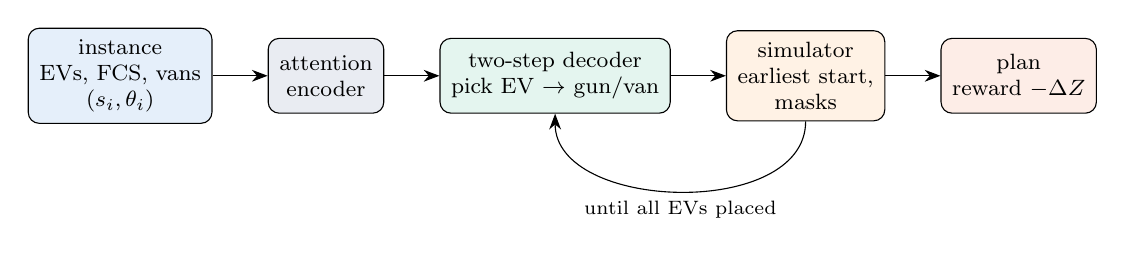
\begin{tikzpicture}[font=\footnotesize,>={Stealth[length=2mm]},
  b/.style={draw,rounded corners,align=center,minimum height=0.95cm,inner sep=4pt},node distance=4mm]
  \node[b,fill=accent!12] (inst) {instance\\ EVs, FCS, vans\\ $(s_i,\theta_i)$};
  \node[b,fill=headblue!10,right=7mm of inst] (enc) {attention\\ encoder};
  \node[b,fill=accent3!12,right=7mm of enc] (dec) {two-step decoder\\ pick EV $\to$ gun/van};
  \node[b,fill=orange!10,right=7mm of dec] (sim) {simulator\\ earliest start,\\ masks};
  \node[b,fill=accent2!12,right=7mm of sim] (rew) {plan\\ reward $-\Delta Z$};
  \draw[->] (inst)--(enc); \draw[->] (enc)--(dec); \draw[->] (dec)--(sim); \draw[->] (sim)--(rew);
  \draw[->] (sim.south) to[out=-90,in=-90] node[below,font=\scriptsize]{until all EVs placed} (dec.south);
\end{tikzpicture}
\caption{The RL policy. The encoder embeds every EV, station and van (including segment and income); the decoder
places EVs one at a time; the simulator schedules each at its earliest feasible time and masks infeasible moves;
the reward is $-\Delta Z$, so the return is $-Z$ (Proposition~\ref{prop:return}).}
\label{fig:rl}
\end{figure}

\textbf{Training.} A generator draws random instances in the style of the data. Each model trains for a
\emph{minimum} of 200 epochs (early stopping is disabled until then), then stops after 10 epochs without a better
validation score, at 500 epochs, or an 8-hour cap --- whichever comes first (Figure~\ref{fig:training}). For an
experiment variant the policy is \emph{retrained} on instances carrying that variant's change, so it is
re-optimised for the new setting, not merely re-applied.

\begin{figure}[H]
\centering
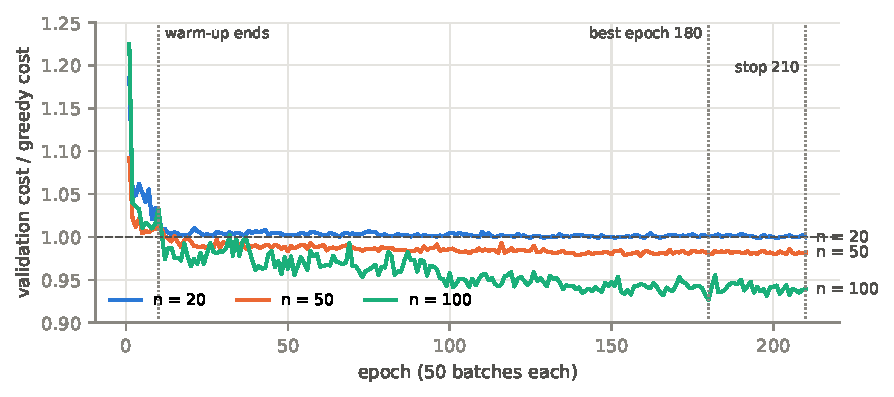
\includegraphics[width=0.86\textwidth]{figures/rl_training.pdf}
\caption{Baseline training: validation cost relative to the greedy rule, by instance size, over epochs
($\frlParams$ parameters, best at epoch \frlBestEpoch).}
\label{fig:training}
\end{figure}

\subsection{Why the two methods are comparable}
Every plan --- from Gurobi, from the greedy rule or from the RL policy --- is written in the same format and scored
by \emph{one} independent checker that re-tests constraints (2)--(23) and recomputes the objective \eqref{eq:obj}.
Neither method is trusted to report its own cost. So a cost difference between the MILP and RL is a real difference
in plan quality, and the $Z$ change an experiment produces can be read off either method and compared
(Section~\ref{sec:milpvsrl}). This shared, neutral yardstick is the backbone of the ``support'' step in every
result below.

\inshort{Gurobi solves the exact model; an attention policy trained with REINFORCE$+$POMO solves it fast, with the
reward set so that maximising return is exactly minimising $Z$ (Proposition~\ref{prop:return}). A single
independent checker scores both, which is what makes the two methods a cross-check on each other.}


\part{Data and baseline results}
%=====================================================================
\section{The data}
\label{sec:data}

The instances are the \textbf{EV-Solomon} set: the 56 Solomon routing files, read as EV-charging instances, at
sizes $n=10,20,\dots,100$ --- $56\times10=560$ instances. Timing is exactly Solomon's (the request is the
``ready time'', the deadline $T$ the depot due date, one grid unit one minute); within a Solomon class the
instances differ only in which cars request when. Each station has 2 guns of 22\,kW, and there are 5 vans.

Onto every EV two attributes are placed, the same number keeping the same pair across a class. The share of
\emph{commercial} cars and the two income distributions are calibrated from Indian data (about \fcomShareData\,\%
commercial among public-charging requests; income drawn from a Beta per segment --- personal skewed rich,
commercial skewed poor). Figure~\ref{fig:data} shows the result.

\begin{figure}[H]
\centering
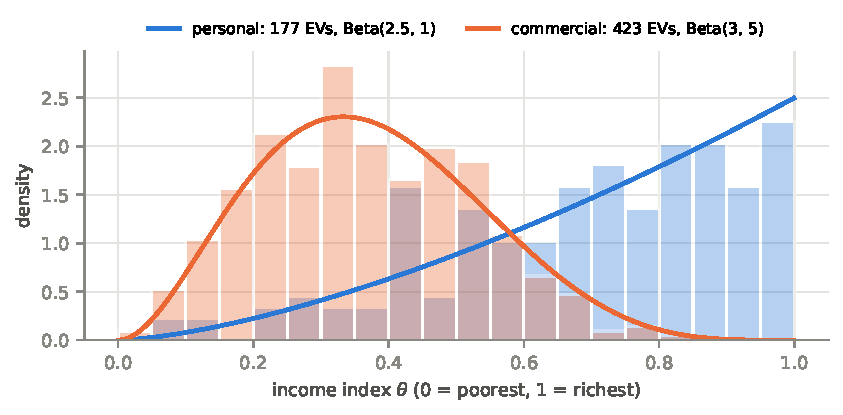
\includegraphics[width=0.82\textwidth]{figures/data_theta.pdf}\\[4pt]
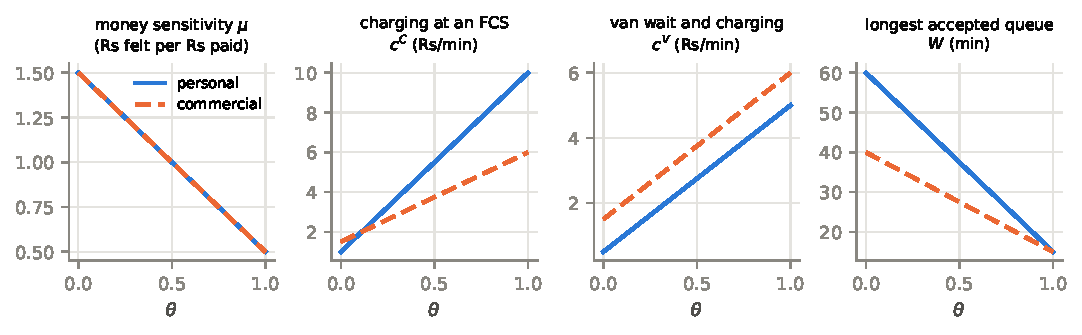
\includegraphics[width=\textwidth]{figures/data_lines.pdf}
\caption{Top: income $\theta$ of the EVs, personal (rich-skewed) and commercial (poor-skewed), with the
calibrated Beta densities. Bottom: how the coefficients move with income --- money felt falls, the value of
station and van time rises, the accepted queue falls; the two segments have different slopes and levels.}
\label{fig:data}
\end{figure}

\begin{table}[H]
\centering
\caption{The six Solomon classes as EV-charging instances (one file per class shown; shared within a class).}
\footnotesize
\begin{adjustbox}{max width=\linewidth}
\begin{tabular}{@{}lrrrrrrrrrr@{}}
\toprule
class & files & $T$ (min) & \shortstack{requests\\at 0 (\%)} & \shortstack{median\\$r/T$ (\%)} & \shortstack{mean $E$\\(kWh)} & \shortstack{stranded\\(\%)} & \shortstack{km to\\nearest FCS} & \shortstack{commercial\\(\%)} & \shortstack{mean $\theta$\\pers.} & \shortstack{mean $\theta$\\comm.} \\
\midrule
C1 & 9 & 1236 & 17 & 22 & 20.5 & 15 & 1.1 & 73 & 0.70 & 0.37 \\
C2 & 8 & 3390 & 19 & 29 & 20.5 & 15 & 1.6 & 69 & 0.72 & 0.39 \\
R1 & 12 & 230 & 25 & 23 & 18.3 & 15 & 1.9 & 70 & 0.64 & 0.37 \\
R2 & 11 & 1000 & 27 & 18 & 18.3 & 15 & 1.9 & 72 & 0.69 & 0.36 \\
RC1 & 8 & 240 & 19 & 25 & 19.9 & 15 & 1.8 & 66 & 0.73 & 0.35 \\
RC2 & 8 & 960 & 19 & 23 & 19.9 & 15 & 1.8 & 73 & 0.68 & 0.35 \\
\bottomrule
\end{tabular}
\end{adjustbox}

\end{table}

\inshort{560 Solomon-timed instances, 10--100 cars. Every car is tagged personal or commercial and given an
income, calibrated so that most public-charging demand is commercial and lower-income --- which is what makes the
segment the decisive variable.}

%=====================================================================
\section{Baseline --- the exact method (MILP)}
\label{sec:basemilp}

\begin{figure}[H]
\centering
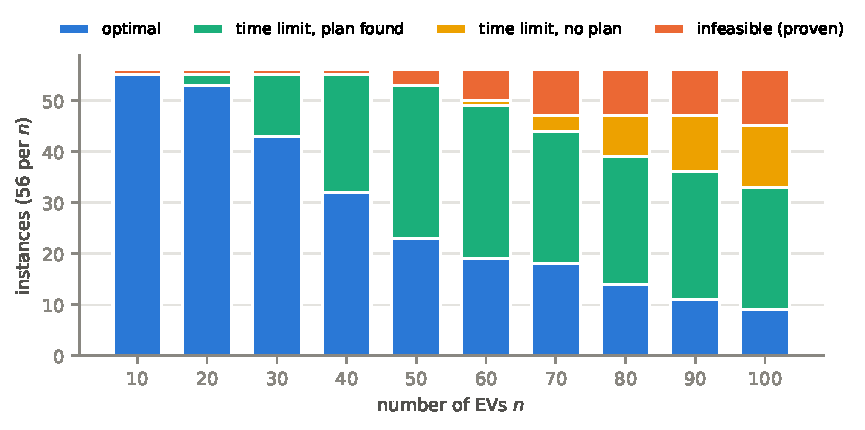
\includegraphics[width=0.86\textwidth]{figures/milp_status_by_n.pdf}
\caption{How the 560 baseline instances ended, by size (56 per size).}
\label{fig:milpstatus}
\end{figure}

\begin{table}[H]
\centering
\caption{MILP baseline by Solomon class. Median gap over the time-limited instances with a plan.}
\small
\begin{adjustbox}{max width=\linewidth}
\begin{tabular}{@{}lrrrrrrrrr@{}}
\toprule
class & instances & optimal & time limit & no plan & infeasible & valid & \shortstack{median\\gap (\%)} & \shortstack{mean\\time (s)} & \shortstack{mean $Z$\\(Rs)} \\
\midrule
C1 & 90 & 66 & 23 & 1 & 0 & 89 & 4.1 & 110 & 47470 \\
C2 & 80 & 56 & 23 & 1 & 0 & 79 & 2.9 & 109 & 47996 \\
R1 & 120 & 41 & 34 & 16 & 29 & 75 & 4.4 & 137 & 32677 \\
R2 & 110 & 70 & 40 & 0 & 0 & 110 & 2.6 & 130 & 44782 \\
RC1 & 80 & 13 & 29 & 16 & 22 & 42 & 7.8 & 171 & 36587 \\
RC2 & 80 & 31 & 48 & 1 & 0 & 79 & 2.9 & 189 & 49691 \\
\bottomrule
\end{tabular}
\end{adjustbox}

\end{table}

\textbf{Result.} \fmilpOptimal{} instances are solved to proven optimality, and \fmilpValid{} have a valid plan
in all; the mean solve time is \fmilpSolveMean\,s. Small instances ($\le20$ cars) are optimal in seconds; from
about 50 cars most hit the 300-second limit. The failures are all in the short-period classes R1 and RC1 at
60--100 cars, where many cars requesting late simply cannot all be charged by $T$ --- the \fmilpInfeasible{}
infeasible instances are \emph{proven} infeasible and are exactly the same set as in formulation~3, so
infeasibility comes from the \emph{data} (time, range, fleet), not from the customer model.

\subsection{What the cost is made of}
\begin{table}[H]
\centering
\caption{The six parts of $Z$ over the valid MILP plans (mean per instance and share).}
\small
\begin{adjustbox}{max width=\linewidth}
\begin{tabular}{@{}lrr@{}}
\toprule
term & mean per instance (Rs) & share of $Z$ (\%) \\
\midrule
$Z_1$ EV driving (perceived) & 388 & 0.9 \\
$Z_2$ van driving & 1067 & 2.4 \\
$Z_3$ van dispatch & 3291 & 7.5 \\
$Z_4$ operator energy & 9204 & 20.9 \\
$Z_5$ tariff (perceived) & 17310 & 39.3 \\
$Z_6$ time (perceived) & 12739 & 29.0 \\
\midrule
$Z$ (all six) & 43999 & 100.0 \\
\bottomrule
\end{tabular}
\end{adjustbox}

\end{table}
The felt tariff $Z_5$ is the largest part (\fshareZFive\,\%) --- every car pays for its energy and most customers
are poor commercial drivers who feel each rupee strongly --- then felt time $Z_6$ (\fshareZSix\,\%) and the
operator's electricity $Z_4$ (\fshareZFour\,\%). Van driving and dispatch are small (\fshareZTwo\,\% and
\fshareZThree\,\%). This split is used later: it is \emph{why} the money-sensitivity and demand levers are the
largest (they scale $Z_5$), and why the van-fleet lever is small (it touches only $Z_2,Z_3$).

\subsection{Who gets a van --- the theory in the data}
\begin{table}[H]
\centering
\caption{The two segments in the baseline plans (MILP and RL). Free-choice cars have a station in range.}
\small
\begin{adjustbox}{max width=\linewidth}
\begin{tabular}{@{}lrrrr@{}}
\toprule
 & personal MILP & personal RL & commercial MILP & commercial RL \\
\midrule
EVs in valid plans & 7043 & 7768 & 16787 & 18282 \\
free-choice EVs & 6095 & 6727 & 14125 & 15418 \\
van share of free-choice EVs (\%) & 19.9 & 6.7 & 0.7 & 0.9 \\
mean $\theta$ & 0.69 & 0.69 & 0.36 & 0.36 \\
mean queue at FCS (min) & 0.41 & 0.79 & 1.58 & 3.36 \\
mean wait for a van (min) & 19.8 & 21.8 & 24.5 & 28.3 \\
mean drive to FCS (min) & 7.8 & 8.3 & 8.9 & 11.3 \\
mean time until charged (min) & 60.6 & 61.8 & 64.3 & 68.3 \\
mean money paid (Rs) & 352 & 332 & 335 & 337 \\
mean time cost (Rs) & 381 & 430 & 200 & 214 \\
mean perceived cost (Rs) & 662 & 699 & 582 & 597 \\
\bottomrule
\end{tabular}
\end{adjustbox}

\end{table}

\begin{figure}[H]
\centering
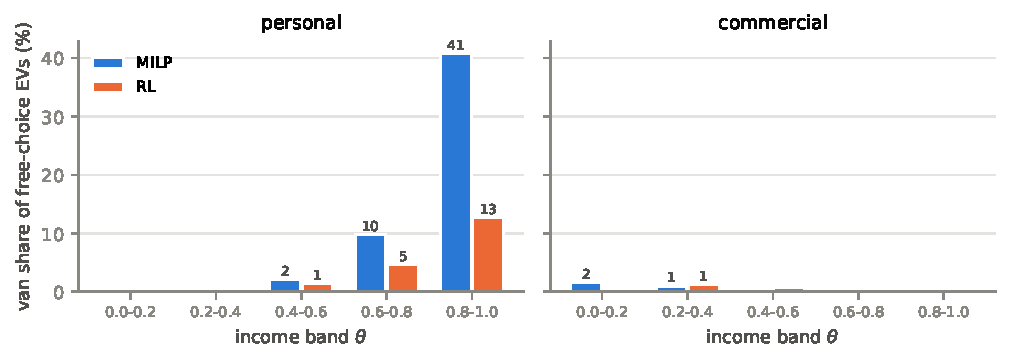
\includegraphics[width=0.95\textwidth]{figures/van_share_income.pdf}
\caption{Share of free-choice cars served by a van, by segment and income band.}
\label{fig:vanincome}
\end{figure}

\begin{table}[H]
\centering
\caption{By income band (MILP). ``Money felt'' is money paid times $\mu$.}
\footnotesize
\begin{adjustbox}{max width=\linewidth}
\begin{tabular}{@{}llrrrrrrr@{}}
\toprule
segment & \shortstack{$\theta$\\band} & EVs & van \% MILP & van \% RL & queue (min) & \shortstack{money\\felt (Rs)} & \shortstack{time cost\\(Rs)} & \shortstack{perceived\\cost (Rs)} \\
\midrule
personal & 0.0-0.2 & 125 & 0.0 & 0.0 & 1.45 & 389 & 120 & 509 \\
 & 0.2-0.4 & 690 & 0.0 & 0.0 & 1.32 & 403 & 243 & 646 \\
 & 0.4-0.6 & 1491 & 2.1 & 1.4 & 0.57 & 338 & 337 & 675 \\
 & 0.6-0.8 & 1934 & 9.8 & 4.7 & 0.18 & 263 & 428 & 691 \\
 & 0.8-1.0 & 2803 & 40.8 & 12.7 & 0.06 & 228 & 418 & 646 \\
\midrule
commercial & 0.0-0.2 & 2532 & 1.6 & 0.5 & 2.77 & 457 & 151 & 607 \\
 & 0.2-0.4 & 7633 & 1.0 & 1.3 & 1.76 & 408 & 186 & 594 \\
 & 0.4-0.6 & 5356 & 0.1 & 0.7 & 0.92 & 333 & 226 & 560 \\
 & 0.6-0.8 & 1186 & 0.0 & 0.5 & 0.75 & 286 & 273 & 559 \\
 & 0.8-1.0 & 80 & 0.0 & 0.0 & 0.00 & 167 & 258 & 425 \\
\bottomrule
\end{tabular}
\end{adjustbox}

\end{table}

The plans are a direct picture of the theory of Section~\ref{sec:theory}:
\begin{itemize}
  \item \textbf{Vans go to personal cars} (\fvanPersMilp\,\% of free-choice personal cars, \fvanComMilp\,\% of
  commercial) --- rule \textbf{(T1)}, the driver-free benefit is for private owners.
  \item \textbf{Among personal cars, van use climbs steeply with income} (0\,\% below $\theta=0.4$, about 41\,\%
  above 0.8); a logistic fit puts the personal threshold at $\theta^{*}\approx\fthetaStarPers$ --- rule
  \textbf{(T3)}.
  \item \textbf{The rare taxi with a van is a \emph{poor} driver with a long queue}, not a rich one --- rule
  \textbf{(T2)}: queues, not income, move taxis to vans. Commercial cars queue \fqueueComMilp{} min on average
  against \fqueuePersMilp{} for personal, so low-income customers absorb the congestion.
\end{itemize}

\support{The \fmilpInfeasible{} infeasible instances match formulation~3's exactly, so feasibility is a property
of the data; and the who-gets-vans pattern is the sign pattern of $\Delta_i$ in \eqref{eq:delP}--\eqref{eq:delC},
not a tuned outcome. The quantitative directions are checked against proven optima in Section~\ref{sec:validation}.}

\inshort{The MILP solves small instances exactly and large ones to within a few per cent; most of the cost is the
felt tariff and felt time; and the plans realise the theory --- vans for rich private owners, stations and queues
for taxis and the poor.}

%=====================================================================
\section{Baseline --- the learning method (RL)}
\label{sec:baserl}

\begin{table}[H]
\centering
\caption{RL against the MILP on the baseline, by class. Gap over instances valid in both.}
\small
\begin{adjustbox}{max width=\linewidth}
\begin{tabular}{@{}lrrrrrrr@{}}
\toprule
class & instances & MILP valid & RL valid & \shortstack{gap mean\\(\%)} & \shortstack{gap median\\(\%)} & MILP s & RL s \\
\midrule
C1 & 90 & 89 & 90 & 0.84 & 0.84 & 110 & 0.12 \\
C2 & 80 & 79 & 79 & 1.66 & 1.80 & 109 & 0.12 \\
R1 & 120 & 75 & 89 & 0.38 & 0.31 & 137 & 0.12 \\
R2 & 110 & 110 & 110 & 1.16 & 1.26 & 130 & 0.12 \\
RC1 & 80 & 42 & 52 & 0.12 & 0.33 & 171 & 0.12 \\
RC2 & 80 & 79 & 80 & 0.48 & 0.46 & 189 & 0.12 \\
\midrule
all & 560 & 474 & 500 & 0.85 & 0.76 & 140 & 0.12 \\
\bottomrule
\end{tabular}
\end{adjustbox}

\end{table}

\begin{figure}[H]
\centering
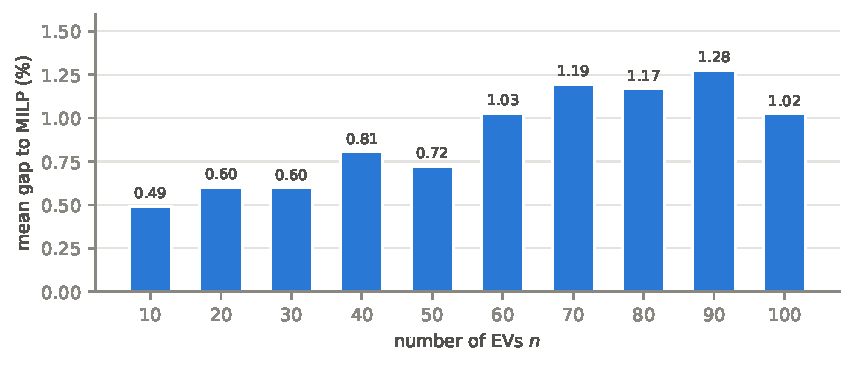
\includegraphics[width=0.82\textwidth]{figures/rl_gap_by_n.pdf}
\caption{Mean cost gap of the RL plan to the MILP, by instance size.}
\label{fig:rlgap}
\end{figure}

\textbf{Result.} The policy finds a valid plan in \frlValid{} instances (MILP \fmilpValid) --- including
\frlOnlyFromNoPlan{} where the MILP's 300-second search found none --- at a mean cost \frlGapMean\,\% above the
MILP (median \frlGapMedian\,\%), in \frlSolveMean\,s per instance against \fmilpSolveMean\,s. Its one weakness is
that it \emph{under-uses vans}: it gives vans to only \fvanPersRl\,\% of free-choice personal cars against the
MILP's \fvanPersMilp\,\%. So the RL cost and the \emph{direction} of its experiment effects are reliable, but its
van shares should not be read as the best policy --- for ``who gets a van'' the MILP is the reference.

\support{RL and the MILP are scored by the same checker (Section~\ref{sec:methods}), so the \frlGapMean\,\% is a
true quality gap, not a reporting artefact. That RL finds plans in \frlOnlyFromNoPlan{} instances the MILP could
not place within the time limit shows the two methods fail in different places, so agreement between them is
strong evidence. Section~\ref{sec:milpvsrl} shows the two methods give the \emph{same} experiment conclusions to
within about \fagreeRtMean{} percentage points.}

\inshort{RL is a fast, robust stand-in: valid plans in \frlValid{} instances, about \frlGapMean\,\% dearer,
roughly a thousand times quicker, and it reproduces the MILP's experiment effects --- but it opens too few vans,
so the exact van policy is read from the MILP.}


\part{The experiments: theory, result, cause, support}
%=====================================================================
\section{The experiments: how to read them}
\label{sec:expintro}

Each experiment changes \emph{one} number in the model (Table~\ref{tab:design}) by a comparable amount, re-solves
all 560 instances, and measures the change against the baseline on the instances feasible in both. E1--E8 are run
by both methods; E9--E10 (Sections~\ref{sec:e9}--\ref{sec:e10}) by the retrained RL policy. Every variant is
presented as \emph{theory} (a proposition read off the model), \emph{result} (the measured table), \emph{practical
cause}, and \emph{support}.

\begin{table}[H]
\centering\small
\caption{The seven experiments and the part of the model each one moves.}
\label{tab:design}
\begin{adjustbox}{max width=\linewidth}
\begin{tabular}{@{}llll@{}}
\toprule
exp. & factor changed & where it enters & variants (baseline) \\
\midrule
E1 & van tariff $p^{\mathrm M}$ & $Z_5$ and the premium $\Pi_i$ \eqref{eq:delP} & 15, 35 Rs/kWh (25) \\
E2 & mobile chargers: vans, seats & fleet $|M|$, seats $Q_m$ in \eqref{eq:vancap} & 3/7 vans, 4/8 seats (5, 6) \\
E5 & value of charging time & $c^{\mathrm C,\mathrm P}$, $\omega$ in $Z_6$ & $\pm25$\,\% \\
E6 & money sensitivity $\mu^{0}$ & $\mu_i$ in $Z_1,Z_5$ (per segment) & $\pm25$\,\% \\
E8 & van battery $B_m$ & battery \eqref{eq:vanbatt} & 200 kWh (150) \\
E9 & station capacity & guns $|G_f|$, power $P^{\mathrm F}$ in \eqref{eq:gunload},\eqref{eq:tau} & 1/4 guns, 11/44 kW (2, 22) \\
E10 & charging demand & energy $E_i$ (everywhere) & $\times0.75,\times1.25$ (1) \\
\bottomrule
\end{tabular}
\end{adjustbox}
\end{table}

\begin{figure}[H]
\centering
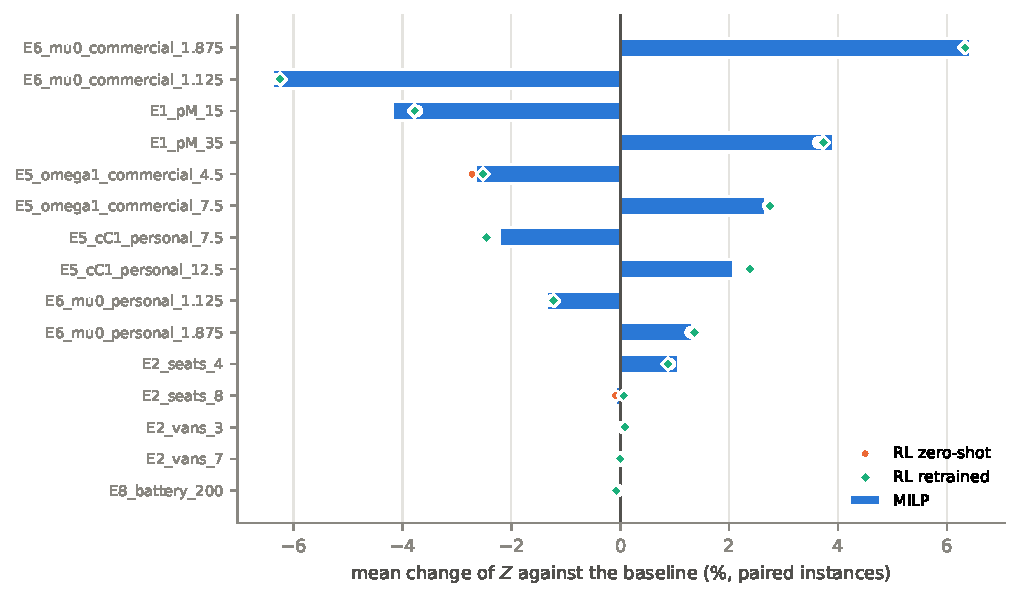
\includegraphics[width=0.9\textwidth]{figures/exp_tornado.pdf}
\caption{Overview: mean change of $Z$ for every E1--E8 variant (bars: MILP; markers: RL zero-shot and retrained),
sorted by size. The two methods land on top of each other.}
\label{fig:tornado}
\end{figure}

%---------------------------------------------------------------------
\subsection{E5 --- the value of charging time}
\label{sec:e5}
E5 raises and lowers, by $\pm25$\,\%, the richest private owner's value of a station minute
($c^{\mathrm C,\mathrm P}$) and the top commercial downtime rate ($\omega^{1}$).

\begin{proposition}[station-time value lifts cost \emph{and} van use for personal cars; downtime rate lifts only cost]
\label{prop:e5}
(a) $\partial Z/\partial c^{\mathrm C,\mathrm P}=\sum_{i\in\mathrm P}\tau^{\mathrm F}_iy_i\cdot\partial c^{\mathrm C,\mathrm P}/\partial(\cdot)\ge0$,
and $\partial\Delta^{\mathrm P}_i/\partial c^{\mathrm C,\mathrm P}=-\tau^{\mathrm F}_i<0$, so a higher personal
value of station time raises $Z$ and makes the van relatively better for personal cars.
(b) Scaling $\omega$ (with $c^{\mathrm D,\mathrm C}=c^{\mathrm C,\mathrm C}=c^{\mathrm V,\mathrm C}=\omega$) multiplies
every commercial time cost, and in $\Delta^{\mathrm C}_i=\mu^{\mathrm C}\Pi_i+\kappa_i-\omega D_i-\delta q^{\mathrm F}_i$
scales only the $\omega D_i$ term, so it changes the cost \emph{level} but barely the commercial assignment.
\end{proposition}
\begin{proof}
(a) $c^{\mathrm C,\mathrm P}$ multiplies $\tau^{\mathrm F}_iy_i$ in $Z_6$ for personal FCS users, a non-negative
quantity, giving the stated sign; it enters $\Delta^{\mathrm P}_i$ \eqref{eq:delP} only through $-c^{\mathrm C,\mathrm P}\tau^{\mathrm F}_i$,
so $\partial\Delta^{\mathrm P}_i/\partial c^{\mathrm C,\mathrm P}=-\tau^{\mathrm F}_i<0$: $\Delta^{\mathrm P}_i$
falls, crossing zero for more cars, so more personal cars take vans. (b) For commercial cars $Z_{6,i}=\omega(C_i-r_i)+\delta q^{\mathrm F}_i$
is linear in $\omega$, so $\partial Z/\partial\omega>0$; in $\Delta^{\mathrm C}_i$ the station and van options are
both priced at $\omega$, so the $\theta$-threshold $\theta^{*}_{i,\mathrm C}$ moves only through the ratio, not the
level --- the choice is first-order invariant.
\end{proof}

\textbf{Result.}
\begin{table}[H]\centering
\caption{E5. Rows: MILP, RL zero-shot, RL retrained. $\Delta$ in \% against the baseline (paired instances).}
\scriptsize
\begin{adjustbox}{max width=\linewidth}
\begin{tabular}{@{}lrrrrrrrrrrr@{}}
\toprule
method & valid & paired & new & lost & \shortstack{$\Delta Z$\\\%} & \shortstack{$\Delta$\\oper. \%} & \shortstack{$\Delta$\\cust. \%} & \shortstack{van \%\\personal} & van \% comm. & vans used & \shortstack{gap to\\MILP \%} \\
\midrule
\multicolumn{12}{@{}l}{\textbf{E5\_cC1\_personal\_7.5}: personal $c^{C,1}$ = 7.5 ($-$25 \%)} \\
MILP & 473 & 472 & 1 & 2 & $-$2.21 & $-$1.15 & $-$2.59 & 19.9 $\to$ 14.1 & 0.7 $\to$ 0.8 & 2.13 & -- \\
RL zero-shot & 499 & 499 & 0 & 1 & $-$2.49 & $-$0.21 & $-$3.45 & 6.7 $\to$ 5.5 & 0.9 $\to$ 0.9 & 2.20 & 0.56 \\
RL retrained & 500 & 499 & 1 & 1 & $-$2.46 & $-$0.59 & $-$3.24 & 6.7 $\to$ 3.9 & 0.9 $\to$ 0.8 & 2.19 & 0.56 \\
\multicolumn{12}{@{}l}{\textbf{E5\_cC1\_personal\_12.5}: personal $c^{C,1}$ = 12.5 ($+$25 \%)} \\
MILP & 473 & 472 & 1 & 2 & $+$2.08 & $+$2.75 & $+$1.84 & 19.9 $\to$ 29.4 & 0.7 $\to$ 0.7 & 2.37 & -- \\
RL zero-shot & 502 & 500 & 2 & 0 & $+$2.45 & $+$0.32 & $+$3.37 & 6.7 $\to$ 8.0 & 0.9 $\to$ 0.8 & 2.23 & 1.22 \\
RL retrained & 500 & 500 & 0 & 0 & $+$2.38 & $+$0.93 & $+$3.02 & 6.7 $\to$ 11.7 & 0.9 $\to$ 0.6 & 2.26 & 1.14 \\
\multicolumn{12}{@{}l}{\textbf{E5\_omega1\_commercial\_4.5}: commercial downtime rate at $\theta=1$: 4.5 ($-$25 \%)} \\
MILP & 472 & 471 & 1 & 3 & $-$2.67 & $-$0.17 & $-$3.80 & 19.9 $\to$ 19.6 & 0.7 $\to$ 0.7 & 2.17 & -- \\
RL zero-shot & 500 & 499 & 1 & 1 & $-$2.72 & $-$0.13 & $-$3.86 & 6.7 $\to$ 6.5 & 0.9 $\to$ 0.8 & 2.19 & 0.82 \\
RL retrained & 500 & 499 & 1 & 1 & $-$2.52 & $+$0.17 & $-$3.69 & 6.7 $\to$ 7.6 & 0.9 $\to$ 0.6 & 2.23 & 0.98 \\
\multicolumn{12}{@{}l}{\textbf{E5\_omega1\_commercial\_7.5}: commercial downtime rate at $\theta=1$: 7.5 ($+$25 \%)} \\
MILP & 475 & 472 & 3 & 2 & $+$2.66 & $+$0.26 & $+$3.81 & 19.9 $\to$ 19.6 & 0.7 $\to$ 0.7 & 2.20 & -- \\
RL zero-shot & 500 & 500 & 0 & 0 & $+$2.72 & $+$0.26 & $+$3.82 & 6.7 $\to$ 6.9 & 0.9 $\to$ 0.9 & 2.24 & 0.83 \\
RL retrained & 499 & 499 & 0 & 1 & $+$2.75 & $+$0.14 & $+$3.92 & 6.7 $\to$ 7.0 & 0.9 $\to$ 0.8 & 2.22 & 0.86 \\
\bottomrule
\end{tabular}
\end{adjustbox}

\end{table}
Personal $c^{\mathrm C,\mathrm P}$ moves $Z$ by about $-2.2$ / $+2.1$\,\% \emph{and} swings the personal van share
(19.9\,\% $\to$ 14.1\,\% when station time is valued less, $\to$ 29.4\,\% when valued more). Commercial $\omega^{1}$
moves $Z$ by about $\pm2.7$\,\% but leaves the van shares unchanged (personal $\approx$19.6\,\%, commercial 0.7\,\%).

\practical{When rich private owners hate station time more, the operator buys them out of the queue with vans ---
so the personal van share rises and the operator's cost goes up with it. A taxi's drive, charge and van minutes
all cost the \emph{same} downtime rate, so raising $\omega$ makes the station \emph{and} the van dearer in lockstep:
the taxi's bill grows but its best option does not change.}

\support{Both methods (MILP and the two RL rows) agree on sign and size. The split outcome --- $c^{\mathrm C,\mathrm P}$
changes the \emph{assignment}, $\omega$ only the \emph{level} --- is exactly Proposition~\ref{prop:e5}, and the van-share
move for $c^{\mathrm C,\mathrm P}$ is visible band-by-band in Figure~\ref{fig:expincome}.}

%---------------------------------------------------------------------
\subsection{E6 --- money sensitivity}
\label{sec:e6}
E6 changes, by $\pm25$\,\%, the poorest customer's money sensitivity $\mu^{0}$, per segment.

\begin{proposition}[the commercial money sensitivity is the strongest cost lever]
\label{prop:e6}
$\mu_i$ multiplies the felt driving $Z_1$ and the felt tariff $Z_5$, so $\partial Z/\partial\mu^{s,0}
=\sum_{i\in s}\big(c^{\mathrm{EV}}\!\sum_f d_{if}Y_{if}+E_i(p^{\mathrm F}y_i+p^{\mathrm M}z_i)\big)\cdot\partial\mu_i/\partial\mu^{s,0}\ge0$.
This is largest for $s=\mathrm C$ because commercial cars are the majority and, being low-income, have $\mu_i$ near
$\mu^{\mathrm C,0}$; and it is small for $s=\mathrm P$ because rich personal cars have $\mu_i$ near the \emph{fixed}
$\mu^{\mathrm P,1}$. The assignment is nearly invariant: $\mu$ scales the station and van tariff together, moving
only the premium term $\mu\Pi_i$ in $\Delta_i$.
\end{proposition}
\begin{proof}
$Z_5=\sum_i\mu_iE_i(p^{\mathrm F}y_i+p^{\mathrm M}z_i)$ and $Z_1$ are linear in each $\mu_i$; by \eqref{eq:lines}
$\partial\mu_i/\partial\mu^{s,0}=(1-\theta_i)\mathbf 1[s_i=s]\ge0$, which is near $1$ for low-income cars and near
$0$ for high-income ones, giving the stated magnitudes. In $\Delta_i$, $\mu$ appears only in $\mu_i\Pi_i$; since
both the FCS and van tariffs scale with $\mu_i$, only the \emph{difference} $\Pi_i=(p^{\mathrm M}-p^{\mathrm F})E_i-c^{\mathrm{EV}}d_{if}$
is re-weighted, a small part of $\Delta_i$, so the chosen resource rarely flips.
\end{proof}

\textbf{Result.}
\begin{table}[H]\centering
\caption{E6. Commercial $\mu^{0}$ is the single largest lever; personal $\mu^{0}$ is minor.}
\scriptsize
\begin{adjustbox}{max width=\linewidth}
\begin{tabular}{@{}lrrrrrrrrrrr@{}}
\toprule
method & valid & paired & new & lost & \shortstack{$\Delta Z$\\\%} & \shortstack{$\Delta$\\oper. \%} & \shortstack{$\Delta$\\cust. \%} & \shortstack{van \%\\personal} & van \% comm. & vans used & \shortstack{gap to\\MILP \%} \\
\midrule
\multicolumn{12}{@{}l}{\textbf{E6\_mu0\_personal\_1.125}: personal $\mu^0$ = 1.125 ($-$25 \%)} \\
MILP & 473 & 472 & 1 & 2 & $-$1.35 & $-$0.01 & $-$1.96 & 19.9 $\to$ 19.8 & 0.7 $\to$ 0.6 & 2.18 & -- \\
RL zero-shot & 500 & 499 & 1 & 1 & $-$1.28 & $+$0.10 & $-$1.89 & 6.7 $\to$ 7.0 & 0.9 $\to$ 0.9 & 2.21 & 0.92 \\
RL retrained & 501 & 500 & 1 & 0 & $-$1.22 & $+$0.07 & $-$1.79 & 6.7 $\to$ 7.8 & 0.9 $\to$ 0.7 & 2.21 & 0.95 \\
\multicolumn{12}{@{}l}{\textbf{E6\_mu0\_personal\_1.875}: personal $\mu^0$ = 1.875 ($+$25 \%)} \\
MILP & 475 & 473 & 2 & 1 & $+$1.33 & $-$0.15 & $+$2.04 & 19.9 $\to$ 18.9 & 0.7 $\to$ 0.7 & 2.18 & -- \\
RL zero-shot & 500 & 499 & 1 & 1 & $+$1.29 & $-$0.03 & $+$1.89 & 6.7 $\to$ 6.5 & 0.9 $\to$ 0.8 & 2.21 & 0.80 \\
RL retrained & 499 & 499 & 0 & 1 & $+$1.36 & $+$0.10 & $+$1.94 & 6.7 $\to$ 7.3 & 0.9 $\to$ 0.8 & 2.22 & 0.84 \\
\multicolumn{12}{@{}l}{\textbf{E6\_mu0\_commercial\_1.125}: commercial $\mu^0$ = 1.125 ($-$25 \%)} \\
MILP & 475 & 474 & 1 & 0 & $-$6.38 & $+$0.05 & $-$9.40 & 19.9 $\to$ 19.6 & 0.7 $\to$ 0.7 & 2.20 & -- \\
RL zero-shot & 499 & 499 & 0 & 1 & $-$6.31 & $+$0.07 & $-$9.18 & 6.7 $\to$ 6.8 & 0.9 $\to$ 0.9 & 2.21 & 0.87 \\
RL retrained & 500 & 500 & 0 & 0 & $-$6.25 & $-$0.12 & $-$9.01 & 6.7 $\to$ 7.1 & 0.9 $\to$ 0.8 & 2.19 & 0.91 \\
\multicolumn{12}{@{}l}{\textbf{E6\_mu0\_commercial\_1.875}: commercial $\mu^0$ = 1.875 ($+$25 \%)} \\
MILP & 475 & 473 & 2 & 1 & $+$6.43 & $+$0.06 & $+$9.47 & 19.9 $\to$ 19.8 & 0.7 $\to$ 0.7 & 2.19 & -- \\
RL zero-shot & 500 & 499 & 1 & 1 & $+$6.34 & $+$0.04 & $+$9.19 & 6.7 $\to$ 6.8 & 0.9 $\to$ 0.9 & 2.21 & 0.80 \\
RL retrained & 500 & 499 & 1 & 1 & $+$6.33 & $+$0.12 & $+$9.15 & 6.7 $\to$ 7.8 & 0.9 $\to$ 0.6 & 2.21 & 0.79 \\
\bottomrule
\end{tabular}
\end{adjustbox}

\end{table}
Commercial $\mu^{0}$ moves $Z$ by $\mp6.4$\,\%, almost all on the customers' side ($\mp9.4$\,\%); personal $\mu^{0}$
moves it only $\pm1.3$\,\%. Van shares stay at about 19--20\,\% (personal) and 0.6--0.7\,\% (commercial) throughout.

\practical{Seven in ten customers are commercial and most are poor, so their money sensitivity multiplies the
biggest slice of the bill --- the tariff ($Z_5$, \fshareZFive\,\% of $Z$). Nudging how a poor taxi driver feels a
rupee therefore swings the whole cost. But it makes the station and the van dearer in the same proportion, so
nobody switches resource.}

\support{The $\pm6.4$\,\% is reproduced by MILP and both RL rows. Its size is predicted by the cost anatomy
(Section~\ref{sec:basemilp}: the tariff is \fshareZFive\,\% of $Z$ and most of it is commercial), and its
near-zero effect on the assignment is Proposition~\ref{prop:e6}.}

%---------------------------------------------------------------------
\subsection{E1 --- the van tariff}
\label{sec:e1}
E1 sets the van tariff $p^{\mathrm M}$ to 15 (no premium over the FCS) and 35 Rs/kWh (baseline 25).

\begin{proposition}[the van tariff is the lever on \emph{who} gets a van]
\label{prop:e1}
A higher $p^{\mathrm M}$ cannot lower the optimal cost, and shrinks the set of EVs assigned to vans:
$\partial Z^{*}/\partial p^{\mathrm M}\ge0$ and $\partial\Delta_i/\partial p^{\mathrm M}=\mu_iE_i>0$, so the
van-choice region $\{\Delta_i<0\}$ contracts as $p^{\mathrm M}$ rises.
\end{proposition}
\begin{proof}
$p^{\mathrm M}$ enters $Z$ only through $Z_5=\sum_i\mu_iE_ip^{\mathrm M}z_i$ with coefficient $\mu_iE_iz_i\ge0$, so
raising it weakly raises the cost of \emph{every} feasible plan and hence the optimum (an envelope/monotonicity
argument: the feasible set is unchanged and the objective rises pointwise). In the margin \eqref{eq:delP}--\eqref{eq:delC},
$p^{\mathrm M}$ appears through $\Pi_i=(p^{\mathrm M}-p^{\mathrm F})E_i-c^{\mathrm{EV}}d_{if}$, so
$\partial\Delta_i/\partial p^{\mathrm M}=\mu_iE_i>0$: each $\Delta_i$ rises, so fewer EVs satisfy $\Delta_i<0$.
\end{proof}

\textbf{Result.}
\begin{table}[H]\centering
\caption{E1. Van tariff $p^{\mathrm M}=15$ (no premium) and 35 Rs/kWh.}
\scriptsize
\begin{adjustbox}{max width=\linewidth}
\begin{tabular}{@{}lrrrrrrrrrrr@{}}
\toprule
method & valid & paired & new & lost & \shortstack{$\Delta Z$\\\%} & \shortstack{$\Delta$\\oper. \%} & \shortstack{$\Delta$\\cust. \%} & \shortstack{van \%\\personal} & van \% comm. & vans used & \shortstack{gap to\\MILP \%} \\
\midrule
\multicolumn{12}{@{}l}{\textbf{E1\_pM\_15}: $p^M$ = 15 Rs/kWh (= $p^F$)} \\
MILP & 471 & 470 & 1 & 4 & $-$4.19 & $+$3.69 & $-$7.80 & 19.8 $\to$ 31.4 & 0.7 $\to$ 1.4 & 2.40 & -- \\
RL zero-shot & 500 & 499 & 1 & 1 & $-$3.74 & $+$0.45 & $-$5.66 & 6.7 $\to$ 8.4 & 0.9 $\to$ 1.0 & 2.22 & 1.31 \\
RL retrained & 499 & 499 & 0 & 1 & $-$3.78 & $+$1.04 & $-$5.97 & 6.7 $\to$ 11.3 & 0.9 $\to$ 1.0 & 2.26 & 1.25 \\
\multicolumn{12}{@{}l}{\textbf{E1\_pM\_35}: $p^M$ = 35 Rs/kWh} \\
MILP & 477 & 474 & 3 & 0 & $+$3.91 & $-$1.39 & $+$6.53 & 19.9 $\to$ 13.5 & 0.7 $\to$ 0.8 & 2.12 & -- \\
RL zero-shot & 499 & 498 & 1 & 2 & $+$3.64 & $-$0.36 & $+$5.49 & 6.7 $\to$ 5.1 & 0.9 $\to$ 0.8 & 2.18 & 0.58 \\
RL retrained & 500 & 499 & 1 & 1 & $+$3.73 & $-$0.76 & $+$5.80 & 6.7 $\to$ 1.1 & 0.9 $\to$ 0.9 & 2.18 & 0.64 \\
\bottomrule
\end{tabular}
\end{adjustbox}

\end{table}
\begin{figure}[H]\centering
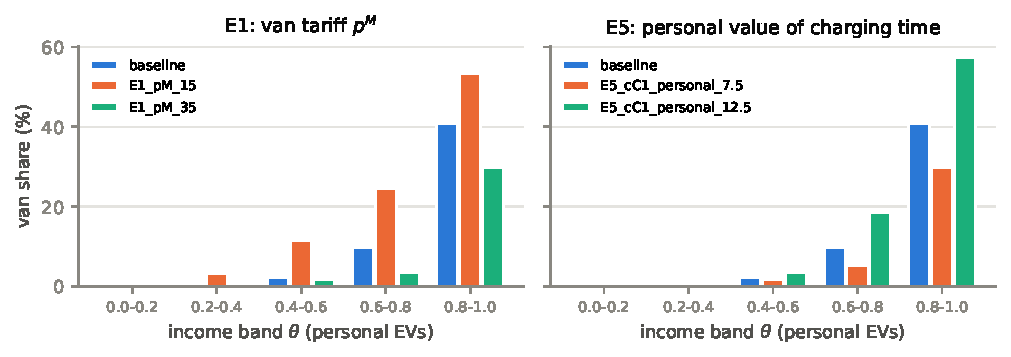
\includegraphics[width=0.95\textwidth]{figures/exp_income.pdf}
\caption{Personal van share by income band: E1 (van tariff) and E5 (personal value of charging time).}
\label{fig:expincome}
\end{figure}
No premium ($p^{\mathrm M}=15$): $Z$ falls about 4.2\,\% --- customers save 7.8\,\%, the operator pays 3.7\,\% more
(more vans dispatched and dearer van energy) --- and the personal van share rises 19.8\,\% $\to$ 31.4\,\%, spreading
down the income scale (Figure~\ref{fig:expincome}). A doubled premium ($35$): $Z$ rises 3.9\,\% and the personal
van share falls to 13.5\,\%.

\practical{The premium is the price of the ``driver-free'' convenience. Cheaper vans let the operator extend that
convenience further down the income scale --- but by rule \textbf{(T1)} the buyers are mostly rich private owners,
so making vans cheaper mostly subsidises them while the operator's own bill goes up.}

\support{Proposition~\ref{prop:e1} forces $\partial Z^{*}/\partial p^{\mathrm M}\ge0$; the direction check
(Section~\ref{sec:validation}) confirms it on the proven optima with zero violations, and the band-by-band shift
of Figure~\ref{fig:expincome} matches the threshold rule \textbf{(T3)}. MILP and RL agree on the cost move and the
direction of the van-share move.}

%---------------------------------------------------------------------
\subsection{E2 --- mobile chargers (fleet size and seats)}
\label{sec:e2}
E2 is the first of the three ``analysis'' factors: the \textbf{number of mobile chargers}. It sets the fleet to 3
or 7 vans (baseline 5) and the seats per van to 4 or 8 (baseline 6).

\begin{proposition}[fleet size buys feasibility, not cost; seats buy cost]
\label{prop:e2}
Enlarging $|M|$ or $Q_m$ only \emph{relaxes} the capacity constraint \eqref{eq:vancap}, so the optimal cost is
non-increasing in both and the feasible set grows. If the fleet is not binding at the optimum, the optimum is
unchanged (only feasibility can change); cutting $Q_m$ tightens \eqref{eq:vancap} and forces more vans to be
dispatched, raising $Z_3$ (and $Z_2$).
\end{proposition}
\begin{proof}
$|M|$ and $Q_m$ appear only on the right-hand side of \eqref{eq:vancap} (and $|M|$ in the routing constraints),
which bound the assignment; increasing them enlarges the feasible region, so $\min Z$ is non-increasing (a larger
feasible set cannot have a higher minimum). By complementary slackness, if \eqref{eq:vancap} is slack at the
optimum a small change of its right-hand side leaves the optimal solution --- and $Z$ --- unchanged; the only
possible change is that a previously infeasible instance becomes feasible. Cutting $Q_m$ removes feasible plans;
serving the same EVs then needs more dispatched vans $u_m$, each adding $c^{\mathrm F}_m$ to $Z_3$.
\end{proof}

\textbf{Result.}
\begin{table}[H]\centering
\caption{E2. 3/7 vans and 4/8 seats. ``new''/``lost'': instances gained/lost against the baseline.}
\scriptsize
\begin{adjustbox}{max width=\linewidth}
\begin{tabular}{@{}lrrrrrrrrrrr@{}}
\toprule
method & valid & paired & new & lost & \shortstack{$\Delta Z$\\\%} & \shortstack{$\Delta$\\oper. \%} & \shortstack{$\Delta$\\cust. \%} & \shortstack{van \%\\personal} & van \% comm. & vans used & \shortstack{gap to\\MILP \%} \\
\midrule
\multicolumn{12}{@{}l}{\textbf{E2\_vans\_3}: 3 vans} \\
MILP & 441 & 441 & 0 & 33 & $-$0.04 & $-$0.53 & $+$0.20 & 19.4 $\to$ 17.4 & 0.2 $\to$ 0.1 & 1.96 & -- \\
RL zero-shot & 465 & 465 & 0 & 35 & $+$0.02 & $-$0.27 & $+$0.15 & 6.4 $\to$ 5.7 & 0.3 $\to$ 0.2 & 2.00 & 0.91 \\
RL retrained & 466 & 466 & 0 & 34 & $+$0.09 & $-$0.12 & $+$0.18 & 6.4 $\to$ 5.9 & 0.4 $\to$ 0.2 & 2.02 & 0.96 \\
\multicolumn{12}{@{}l}{\textbf{E2\_vans\_7}: 7 vans} \\
MILP & 487 & 474 & 13 & 0 & $+$0.02 & $+$0.22 & $-$0.05 & 19.9 $\to$ 20.5 & 0.7 $\to$ 0.7 & 2.22 & -- \\
RL zero-shot & 506 & 500 & 6 & 0 & $+$0.04 & $+$0.13 & $+$0.03 & 6.7 $\to$ 6.7 & 0.9 $\to$ 1.0 & 2.23 & 0.84 \\
RL retrained & 506 & 500 & 6 & 0 & $+$0.00 & $+$0.06 & $-$0.00 & 6.7 $\to$ 7.0 & 0.9 $\to$ 0.7 & 2.23 & 0.81 \\
\multicolumn{12}{@{}l}{\textbf{E2\_seats\_4}: 4 EVs per van} \\
MILP & 471 & 467 & 4 & 7 & $+$1.08 & $+$3.03 & $+$0.26 & 19.8 $\to$ 11.6 & 0.3 $\to$ 0.2 & 2.48 & -- \\
RL zero-shot & 493 & 493 & 0 & 7 & $+$0.91 & $+$3.87 & $-$0.35 & 6.7 $\to$ 5.8 & 0.5 $\to$ 0.4 & 2.54 & 0.69 \\
RL retrained & 494 & 494 & 0 & 6 & $+$0.88 & $+$4.04 & $-$0.46 & 6.8 $\to$ 7.2 & 0.5 $\to$ 0.3 & 2.55 & 0.65 \\
\multicolumn{12}{@{}l}{\textbf{E2\_seats\_8}: 8 EVs per van} \\
MILP & 471 & 471 & 0 & 3 & $-$0.08 & $-$0.28 & $+$0.06 & 19.9 $\to$ 21.6 & 0.7 $\to$ 0.8 & 2.13 & -- \\
RL zero-shot & 500 & 499 & 1 & 1 & $-$0.08 & $-$0.61 & $+$0.16 & 6.7 $\to$ 6.6 & 0.9 $\to$ 0.9 & 2.13 & 0.85 \\
RL retrained & 499 & 499 & 0 & 1 & $+$0.07 & $-$0.31 & $+$0.25 & 6.7 $\to$ 7.2 & 0.9 $\to$ 0.9 & 2.16 & 0.98 \\
\bottomrule
\end{tabular}
\end{adjustbox}

\end{table}
\begin{figure}[H]\centering
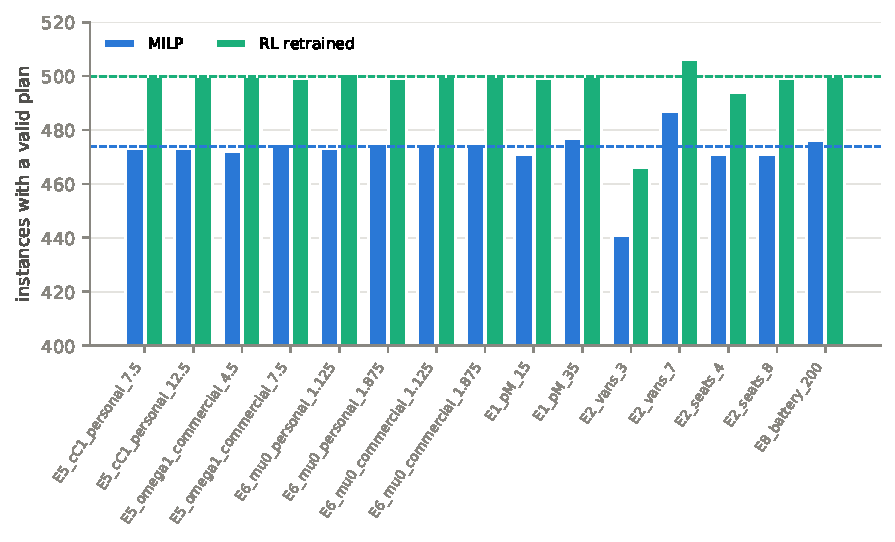
\includegraphics[width=0.95\textwidth]{figures/exp_valid.pdf}
\caption{Instances with a valid plan per variant (MILP vs RL retrained); dashed lines are the baseline.}
\label{fig:expvalid}
\end{figure}
On instances optimal in both runs the cost change from the fleet size is \textbf{0.000\,\%} (Table~\ref{tab:direction}):
the plans use only about 2.2 vans, so the fifth is rarely needed for cost. But 3 vans lose 33 instances and 7 vans
gain 13 --- almost all large R1/RC1 instances (Figure~\ref{fig:expvalid}). Cutting seats to 4 raises $Z$ about
1.1\,\% (1.3\,\% at the optima) and drops the personal van share 19.8\,\% $\to$ 11.6\,\%.

\practical{Extra vans sit idle on easy instances --- the baseline fleet already covers the demand --- so they do
not lower the bill; they earn their keep only on the hard, short-period instances where many stranded or late cars
need van trips at once. Fewer seats, by contrast, bite everywhere: the operator must send out more vans to carry
the same cars, and each dispatch is a fixed cost.}

\support{Proposition~\ref{prop:e2} predicts exactly the observed split (0.000\,\% at the optima, but
feasibility moving), and the direction check records zero cost violations. The feasibility gains/losses concentrate
in R1/RC1 as the short-period theory requires, and MILP and RL agree.}

%---------------------------------------------------------------------
\subsection{E8 --- the van battery}
\label{sec:e8}
E8 raises the van battery to 200 kWh (baseline 150).

\begin{proposition}[a slack battery has no effect]
\label{prop:e8}
Raising $B_m$ relaxes \eqref{eq:vanbatt}, so $\min Z$ is non-increasing; if the battery is slack at the optimum
(seats or time bind first), the optimum --- and $Z$ --- is unchanged.
\end{proposition}
\begin{proof}
$B_m$ is the right-hand side of \eqref{eq:vanbatt}; increasing it enlarges the feasible set, so $\min Z$ is
non-increasing. By complementary slackness, a slack constraint's multiplier is zero, so a marginal change of
$B_m$ does not move the optimum.
\end{proof}

\textbf{Result.}
\begin{table}[H]\centering
\caption{E8. Van battery 200 kWh instead of 150.}
\scriptsize
\begin{adjustbox}{max width=\linewidth}
\begin{tabular}{@{}lrrrrrrrrrrr@{}}
\toprule
method & valid & paired & new & lost & \shortstack{$\Delta Z$\\\%} & \shortstack{$\Delta$\\oper. \%} & \shortstack{$\Delta$\\cust. \%} & \shortstack{van \%\\personal} & van \% comm. & vans used & \shortstack{gap to\\MILP \%} \\
\midrule
\multicolumn{12}{@{}l}{\textbf{E8\_battery\_200}: B = 200 kWh} \\
MILP & 476 & 473 & 3 & 1 & $-$0.01 & $-$0.40 & $+$0.19 & 19.9 $\to$ 18.5 & 0.7 $\to$ 0.7 & 2.14 & -- \\
RL zero-shot & 501 & 500 & 1 & 0 & $-$0.02 & $-$0.17 & $+$0.05 & 6.7 $\to$ 6.5 & 0.9 $\to$ 0.9 & 2.19 & 0.83 \\
RL retrained & 500 & 499 & 1 & 1 & $-$0.07 & $-$0.06 & $-$0.07 & 6.7 $\to$ 8.2 & 0.9 $\to$ 0.7 & 2.18 & 0.77 \\
\bottomrule
\end{tabular}
\end{adjustbox}

\end{table}
$Z$ changes by $-0.01$\,\% on average ($-0.04$\,\% at the optima): the battery almost never binds --- seats and
time run out first. By the rule fixed before the run (an effect below 1\,\% is negligible), \textbf{van recharging
need not be modelled}.

\practical{In a one-period plan a van makes a handful of stops; its seats and the deadline cap the route long
before its battery would. So a bigger tank changes nothing the operator can use.}

\support{Proposition~\ref{prop:e8} predicts the near-zero effect from complementary slackness; the direction check
confirms a weak decrease with no violation, and both methods report essentially 0\,\%.}

%=====================================================================
\section{Station capacity (E9): guns per station and power per gun}
\label{sec:e9}

Station capacity is the second of the three factors the course asks the analysis to study (the first, the number of mobile chargers, is E2, covered earlier in this Part). A fixed charging station (FCS) has two capacity knobs:
\begin{itemize}
  \item \textbf{guns} (charging points) per station: how many cars a station can charge \emph{at the same time};
  \item \textbf{power} per gun (kW): how \emph{fast} each car charges.
\end{itemize}
The baseline has 2 guns of 22\,kW at each station. Experiment E9 halves and doubles each knob on its own: 1 or 4 guns, 11 or 44\,kW. Every variant is solved by reinforcement learning with a model \emph{retrained} for that setting (there is no MILP for E9/E10; the RL policy, shown throughout this report to track the MILP closely, is used as the fast, faithful tool). The four variants are measured against the baseline RL plan on the instances where both are feasible.

\begin{figure}[H]
\centering
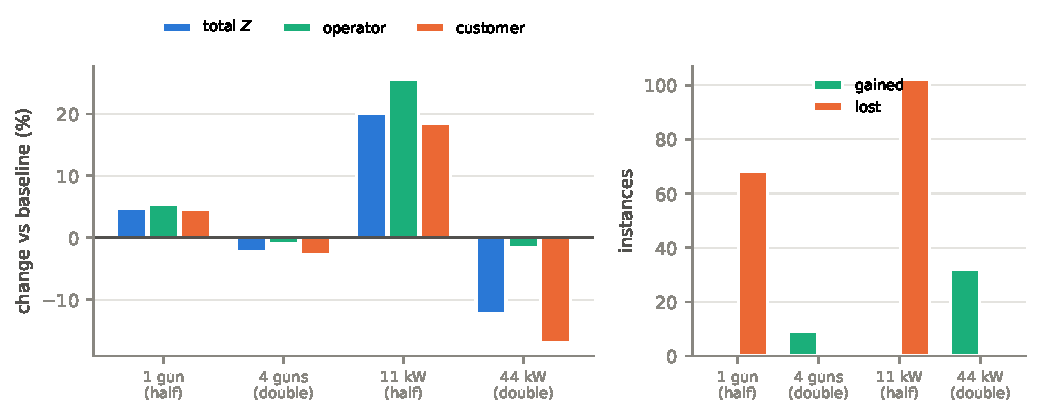
\includegraphics[width=\textwidth]{figures/exp_e9.pdf}
\caption{E9 station capacity. Left: change of the total cost $Z$ and of its operator and customer parts against the baseline (\%, paired instances). Right: instances that gain or lose a feasible plan.}
\label{fig:e9}
\end{figure}

\begin{table}[H]
\centering
\caption{E9, retrained RL. ``comm.\ queue'' and ``van \% pers.'' are shown baseline $\to$ variant. ``gained''/``lost'': instances that become feasible / infeasible. ``paired'': instances feasible in both.}
\scriptsize
\begin{adjustbox}{max width=\linewidth}
\begin{tabular}{@{}llrrrllrrr@{}}
\toprule
variant & what changes & \shortstack{$\Delta Z$\\\%} & \shortstack{$\Delta$\\oper. \%} & \shortstack{$\Delta$\\cust. \%} & \shortstack{comm. queue\\(min)} & van \% pers. & gained & lost & paired \\
\midrule
E9\_guns\_1 & 1 gun per station (half) & $+$4.76 & $+$5.40 & $+$4.55 & 1.18 $\to$ 3.48 & 6.2 $\to$ 16.7 & 0 & 68 & 432 \\
E9\_guns\_4 & 4 guns per station (double) & $-$2.21 & $-$0.90 & $-$2.72 & 2.50 $\to$ 0.53 & 6.7 $\to$ 5.3 & 9 & 0 & 500 \\
E9\_power\_11 & 11 kW per gun (half) & $+$20.13 & $+$25.61 & $+$18.43 & 1.25 $\to$ 0.77 & 6.3 $\to$ 58.7 & 0 & 102 & 398 \\
E9\_power\_44 & 44 kW per gun (double) & $-$12.30 & $-$1.54 & $-$16.97 & 2.50 $\to$ 2.32 & 6.7 $\to$ 0.0 & 32 & 0 & 500 \\
\bottomrule
\end{tabular}
\end{adjustbox}

\end{table}

\subsection{What the numbers say}
\begin{itemize}
  \item \textbf{Power is the strong lever, guns the weak one.} Halving the power to 11\,kW changes $Z$ by \feNinePowHalfDz\,\%; doubling it to 44\,kW by $-$\feNinePowDblDzAbs\,\%. Halving or doubling the \emph{guns} moves $Z$ only by \feNineGunsHalfDz\,\% and $-$\feNineGunsDblDzAbs\,\%.
  \item \textbf{The two knobs act through different channels.} Fewer guns triple the commercial queue (\feNineGunsHalfQBase{} $\to$ \feNineGunsHalfQ{} min): with one gun the cars at a station must wait their turn. Lower power barely changes the queue; instead it makes station charging so slow that charging moves onto the vans --- the personal van share jumps from about 6\,\% to \feNinePowHalfVan\,\%.
  \item \textbf{Capacity decides feasibility.} Weaker capacity strands cars that can no longer be charged before the deadline: \feNinePowHalfLost{} instances lose a feasible plan at 11\,kW and \feNineGunsHalfLost{} at 1~gun. Stronger capacity rescues some: \feNinePowDblGain{} at 44\,kW, \feNineGunsDblGain{} at 4~guns.
\end{itemize}

\inshort{Power per gun is the dominant capacity lever (about $\pm$12--20\,\% on $Z$); the number of guns matters much less (about $\pm$2--5\,\%) and only through queueing. Cutting capacity also strands dozens of instances.}

\subsection{Why: the charging-time law}

\begin{figure}[H]
\centering
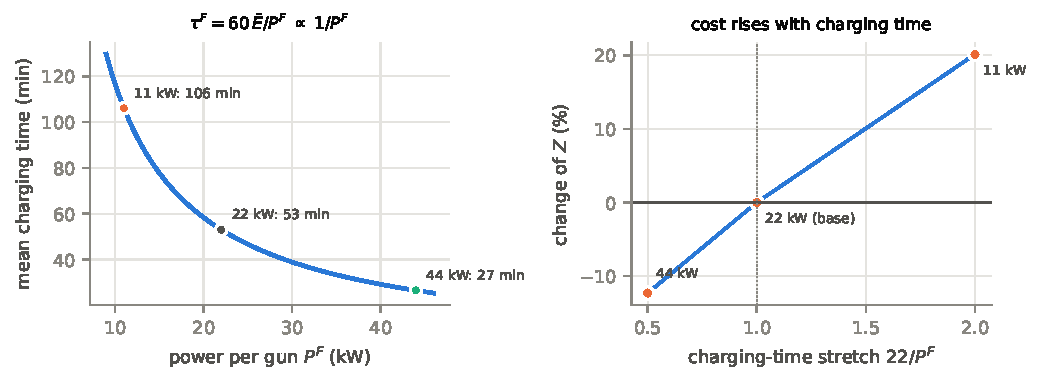
\includegraphics[width=\textwidth]{figures/exp_e9_power.pdf}
\caption{Left: FCS charging time against power per gun --- an inverse law. Right: the measured change of $Z$ rises with the charging-time ``stretch'' $22/P^F$.}
\label{fig:e9power}
\end{figure}

The whole pattern follows from one identity in the model.

\begin{keybox}
\textbf{Proposition 1 (charging-time law).} The time an EV $i$ spends charging at an FCS is
\[
\tau^F_i \;=\; \frac{60\,E_i}{P^F}\quad\text{minutes},
\]
where $E_i$ is its energy demand (kWh) and $P^F$ the power per gun (kW). Hence $\tau^F_i \propto 1/P^F$: scaling the power by a factor $\rho$ scales \emph{every} FCS charging time by $1/\rho$.\\[2pt]
\textbf{Proof.} Energy $=$ power $\times$ time, so the charging time in hours is $E_i/P^F$; $\times 60$ gives minutes. The power $P^F$ appears only in the denominator, so $\tau^F_i$ is inversely proportional to it. $\square$
\end{keybox}

With the mean demand $\bar E \approx \fmeanEnergy$\,kWh, the baseline charging time is $\tau^F=\feNineTauBase$\,min; halving the power doubles it to \feNineTauHalf\,min, doubling it halves it to \feNineTauDbl\,min (Figure~\ref{fig:e9power}, left). Power changes the \emph{time} a car charges, not the \emph{energy} it draws, so the operator's electricity bill ($Z_4$) is untouched; what moves is every time-cost term that contains $\tau^F$.

\begin{keybox}
\textbf{Proposition 2 (power is first order, guns are second order).} Write the customers' charging-time cost as $Z_{\text{chg}}=\sum_i c^C_i\,\tau^F_i=\dfrac{60}{P^F}\sum_i c^C_i E_i$, a part of $Z_6$. Then $Z_{\text{chg}}\propto 1/P^F$, so power acts on this large term directly. The number of guns does \emph{not} enter $\tau^F_i$; it only sets how many cars may charge in parallel at a station (the gun-load constraint), and so changes $Z$ only through the queue term $\sum_i c^Q_i\,\tau^Q_i$. Because the mean queue ($\approx$1--2\,min) is far smaller than the mean charging time ($\feNineTauBase$\,min), $\bigl|\partial Z/\partial(\text{power})\bigr|\gg\bigl|\partial Z/\partial(\text{guns})\bigr|$.\\[2pt]
\textbf{Proof.} $P^F$ enters the objective only through $\tau^F_i=60E_i/P^F$ in the charging-time terms, giving the stated $1/P^F$ law. The gun count enters only the per-station capacity constraint (at most ``guns'' cars charging at once), which bounds the queueing delay $\tau^Q_i$ but leaves $\tau^F_i$, $E_i$ and the tariff unchanged. The size of each lever is the size of the term it scales; charging time dominates queueing time in the data by more than an order of magnitude. $\square$
\end{keybox}

This is exactly what the experiment shows: power moves $Z$ by $\pm$12--20\,\%, guns by $\pm$2--5\,\%, and the guns variants move the \emph{queue} while the power variants move the \emph{van share}.

\textbf{Why the van share explodes at low power.} When the FCS takes \feNineTauHalf\,minutes, station charging becomes so slow that a van --- which charges a car wherever it stands, with no station queue and no driver waiting --- becomes worth its premium even for private owners who would normally use a station. The policy therefore sends \feNinePowHalfVan\,\% of free-choice personal cars to vans (against about 6\,\% at the baseline). At 44\,kW the station is so fast (\feNineTauDbl\,min) that the van's advantage disappears and the personal van share falls to~0. The van is the model's release valve for expensive station time: the clearest possible sign that FCS charging time is the binding cost.

\begin{keybox}
\textbf{Proposition 3 (the effect is asymmetric, by convexity).} Under power $P^F\!\to\!\rho P^F$ the charging time changes by $\Delta\tau=\tau^F(1/\rho-1)$. Because $\tau^F(P)\propto 1/P$ is convex, halving the power ($\rho=\tfrac12$) \emph{adds} $\tau^F$ minutes ($+\feNineTauBase$) while doubling it ($\rho=2$) \emph{removes} only $\tau^F/2$ ($-\!\approx\!27$). Hence the cost rise from halving exceeds the cost fall from doubling, as observed ($+\feNinePowHalfDz$\,\% vs $-$\feNinePowDblDzAbs\,\%).\\[2pt]
\textbf{Proof.} $\tau^F(\rho P)=\tau^F(P)/\rho$, so $\Delta\tau(\rho=\tfrac12)=\tau^F$ and $\Delta\tau(\rho=2)=-\tau^F/2$; $|\!+\!\tau^F|>|\!-\!\tau^F/2|$. The cost terms are increasing in $\tau^F$, so their change inherits this inequality. The asymmetry is reinforced by the deadline $C_i\le T$: at half power the completion time binds for many cars (\feNinePowHalfLost{} become infeasible and the survivors pay heavily), whereas at double power the deadline is already slack, so the extra speed has no value once a car is charged in time --- the benefit saturates. $\square$
\end{keybox}

\inshort{One identity, $\tau^F=60E/P^F$, explains E9. Power scales the dominant charging-time cost as $1/P^F$ (a convex, hence asymmetric, law) and, when low enough, pushes charging onto vans; guns touch only the small queue term. Below a point, cutting capacity makes instances infeasible rather than merely dearer.}

%=====================================================================
\section{Charging demand (E10): energy per car}
\label{sec:e10}

Charging demand is the third factor the analysis must cover. ``Demand'' has two meanings, and the study separates them:
\begin{itemize}
  \item \textbf{how many cars} --- this is the size sweep $n=10,20,\dots,100$ that every experiment already runs, so its effect is visible throughout the report;
  \item \textbf{how much energy each car needs} --- this is what E10 changes, scaling every EV's energy demand $E_i$ by a factor $s=0.75$ and $s=1.25$ ($\pm25$\,\%) and retraining the policy for each.
\end{itemize}
A larger $E_i$ lengthens every charging session (at a station and in a van), draws more electricity and raises every per-kWh charge, so more energy per car should tighten the stations and the vans and raise the cost; less should do the reverse.

\begin{figure}[H]
\centering
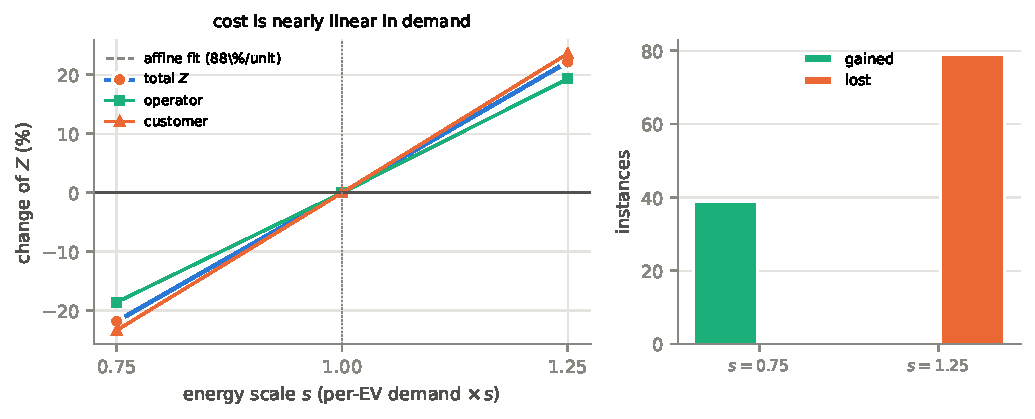
\includegraphics[width=\textwidth]{figures/exp_e10.pdf}
\caption{E10 charging demand. Left: change of $Z$ (and its operator/customer parts) against the energy scale $s$; the dashed line is the affine fit through the baseline. Right: instances that gain or lose a feasible plan.}
\label{fig:e10}
\end{figure}

\begin{table}[H]
\centering
\caption{E10, retrained RL. The baseline is $s=1$ (no change).}
\footnotesize
\begin{adjustbox}{max width=\linewidth}
\begin{tabular}{@{}llrrrrrr@{}}
\toprule
variant & what changes & \shortstack{$\Delta Z$\\\%} & \shortstack{$\Delta$\\oper. \%} & \shortstack{$\Delta$\\cust. \%} & gained & lost & paired \\
\midrule
E10\_demand\_0.75 & energy per EV x0.75 ($-$25 \%) & $-$21.82 & $-$18.59 & $-$23.35 & 39 & 0 & 500 \\
E10\_demand\_1.25 & energy per EV x1.25 ($+$25 \%) & $+$22.19 & $+$19.33 & $+$23.57 & 0 & 79 & 421 \\
\bottomrule
\end{tabular}
\end{adjustbox}

\end{table}

\subsection{What the numbers say}
\begin{itemize}
  \item \textbf{The response is large and nearly symmetric}: $-25$\,\% energy moves $Z$ by $-$\feTenDownDzAbs\,\%, $+25$\,\% moves it by \feTenUpDz\,\%. Operator cost and customer cost move together and in the same proportion.
  \item \textbf{It is nearly linear}: the three points ($s=0.75,1,1.25$) sit almost on a straight line through the baseline (Figure~\ref{fig:e10}, left), with a slope of about \feTenSlope\,\% per unit of~$s$.
  \item \textbf{Feasibility moves too}: $+25$\,\% energy strands \feTenUpLost{} instances (longer sessions miss the deadline), $-25$\,\% rescues \feTenDownGain.
\end{itemize}

\inshort{Charging demand is the single most powerful of the three analysis factors for the cost: a $\pm25$\,\% change in energy per car moves $Z$ by about $\pm22$\,\%, almost one-for-one.}

\subsection{Why: the cost is affine in demand}

\begin{keybox}
\textbf{Proposition 4 (energy affinity).} Scale every EV's energy demand by $s$: $E_i\!\to\! sE_i$. Then the total cost is affine in $s$,
\[
Z(s)=a+b\,s,
\]
where $b$ collects the terms proportional to the energies and $a$ the terms independent of them.\\[2pt]
\textbf{Proof.} Each objective term is one of two kinds. \emph{Energy-proportional} (each scales by $s$ when all $E_i$ do): the FCS charging time $\tau^F_i=60sE_i/P^F$ and the van charging time, so their time-costs; the operator's electricity $Z_4=\pi\sum_i sE_i$; the perceived tariff $Z_5=\sum_i \mu_i\,p\,sE_i$. \emph{Energy-independent}: van driving $Z_2$ (road distance), van dispatch $Z_3$ (a fixed cost per van used), and the drive-to-station time inside $Z_6$ (set by geometry, not by $E_i$). Summing a group that scales linearly with $s$ and a group that does not gives $Z(s)=bs+a$. $\square$
\end{keybox}

\begin{keybox}
\textbf{Corollary (elasticity and symmetry).} The elasticity of cost to demand at the baseline is
\[
\varepsilon=\left.\frac{dZ/Z}{ds/s}\right|_{s=1}=\frac{b}{a+b},
\qquad\text{so}\qquad
\frac{\Delta Z}{Z}(s)=\varepsilon\,(s-1).
\]
Hence the percentage change is a straight line through the baseline with slope $100\,\varepsilon$, and equal-and-opposite for $\pm\delta$. Measured slope $\approx\feTenSlope$ gives $\varepsilon\approx\feTenElastic$: about \feTenElastic{} of the cost scales directly with energy.\\[2pt]
\textbf{Proof.} From $Z(s)=a+bs$, $Z(1)=a+b$ and $\Delta Z/Z=(Z(s)-Z(1))/Z(1)=b(s-1)/(a+b)=\varepsilon(s-1)$; the slope in $s$ is $100\varepsilon$ and $\Delta Z/Z(1\pm\delta)=\pm\varepsilon\delta$ is symmetric. $\square$
\end{keybox}

The elasticity is below~1 because a share $a/(a+b)=1-\varepsilon\approx\feTenNonElastic\,\%$ of the cost does \emph{not} scale with energy. The baseline cost breakdown names this share almost exactly: van driving ($Z_2$, \fshareZTwo\,\%) and dispatch ($Z_3$, \fshareZThree\,\%) are purely geometric, and together with the fixed drive-to-station time they make up the roughly \feTenNonElastic\,\% that stays put while everything else --- the tariff ($Z_5$, \fshareZFive\,\%), the operator energy ($Z_4$, \fshareZFour\,\%) and the charging-time cost --- grows with $s$. The small departure from perfect symmetry ($-$\feTenDownDzAbs\,\% vs \feTenUpDz\,\%) is not a failure of the theory: it comes from the feasible set itself changing with $s$ (\feTenUpLost{} instances lost at $s=1.25$ against \feTenDownGain{} gained at $s=0.75$), so the two sides are averaged over slightly different instances.

\subsection{The three analysis factors side by side}

With E9 and E10 in hand, the three factors the course asks about can be ranked by their effect on the cost $Z$:
\begin{enumerate}
  \item \textbf{Charging demand (E10)}: $\pm25$\,\% energy $\Rightarrow$ about $\pm22$\,\% on $Z$ (elasticity \feTenElastic). The strongest lever, because most of $Z$ is energy-proportional.
  \item \textbf{Station power (E9)}: halving/doubling $\Rightarrow$ $+\feNinePowHalfDz$\,\% / $-$\feNinePowDblDzAbs\,\%, through the charging-time law $\tau^F\propto1/P^F$.
  \item \textbf{Mobile chargers (E2)}: the fleet \emph{size} barely touches the cost (about 0\,\% at the optima) and acts almost entirely on feasibility; cutting seats per van costs about $+1.3$\,\%.
  \item \textbf{Station guns (E9)}: $+\feNineGunsHalfDz$\,\% / $-$\feNineGunsDblDzAbs\,\%, the weakest cost lever, acting only through queueing.
\end{enumerate}
All three factors, however, share one role that the cost figures hide: at the hard end they decide \emph{feasibility}. Too little energy headroom, too few guns, too little power or too small a fleet each strand cars that cannot be charged before the deadline --- which is why every variant above also shows instances gained or lost.

\inshort{Because about \feTenElastic{} of $Z$ is proportional to the energy charged, the cost is essentially linear in demand and demand is the biggest single lever; station power is next (a convex $1/P$ law), the van fleet and the gun count move the cost little but govern feasibility.}


\part{Synthesis, validation and conclusions}
%=====================================================================
\section{Which assumption matters most}
\label{sec:ranking}

Putting all seven experiments on one scale answers the operator's real question: where is it worth spending effort
to measure a number well, or money to change it?

\textbf{Effect on the total cost $Z$} (a $\pm25$\,\% or comparable change), largest first:
\begin{enumerate}[itemsep=1pt]
  \item \textbf{Charging demand} (E10): about $\pm22$\,\% --- most of $Z$ is energy-proportional (elasticity \feTenElastic);
  \item \textbf{Station power} (E9): $+\feNinePowHalfDz$ / $-$\feNinePowDblDzAbs\,\% --- the convex $\tau^{\mathrm F}\propto1/P^{\mathrm F}$ law;
  \item \textbf{Commercial money sensitivity} $\mu^{0}$ (E6): $\pm6.4$\,\% --- it weights the dominant tariff term for the majority segment;
  \item \textbf{Van tariff} $p^{\mathrm M}$ (E1): $-4.2$ / $+3.9$\,\%;
  \item \textbf{Station guns} (E9): $+\feNineGunsHalfDz$ / $-$\feNineGunsDblDzAbs\,\% --- queueing only;
  \item \textbf{Commercial downtime} $\omega$ (E5): $\pm2.7$\,\%; \textbf{personal value of station time} $c^{\mathrm C,\mathrm P}$ (E5): $\pm2.1$\,\%;
  \item \textbf{Personal money sensitivity} (E6): $\pm1.3$\,\%; \textbf{seats per van} (E2, cut only): $+1.1$\,\%;
  \item \textbf{Number of vans} (E2) and \textbf{van battery} (E8): about $0$\,\% --- but the fleet governs feasibility.
\end{enumerate}

\textbf{Effect on \emph{who} gets a van} is a different ranking: the van tariff, the personal value of station time
and cutting seats swing the personal van share by 6--12 points (and station power by tens of points); the money
sensitivities, the downtime rate and the battery barely touch it (Figure~\ref{fig:vanshare}).

\begin{figure}[H]
\centering
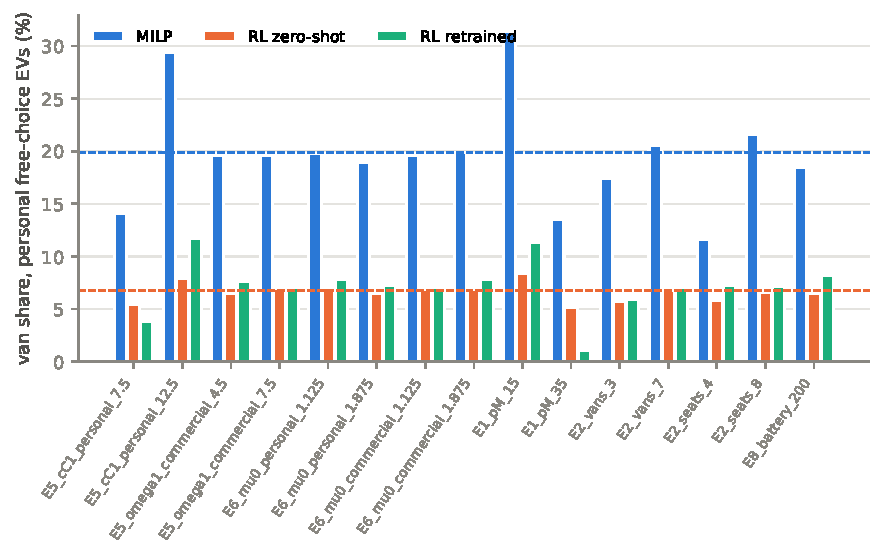
\includegraphics[width=0.95\textwidth]{figures/exp_vanshare.pdf}
\caption{Personal van share for every E1--E8 variant (MILP, RL zero-shot, RL retrained); dashed lines are the
baseline. Levers of price and of personal time move it; levers of money sensitivity and downtime do not.}
\label{fig:vanshare}
\end{figure}

\inshort{To estimate the \emph{cost}, the energy per car, the station power and how poor taxi drivers feel money
matter most. To decide \emph{who gets a van}, the van tariff and the personal value of station time are the tools;
the fleet size and battery decide only which instances can be served at all.}

%=====================================================================
\section{Validation: why the numbers can be trusted}
\label{sec:validation}

The report rests on three independent kinds of support, over and above each proposition's derivation.

\subsection{A direction the optimiser cannot violate}
Some directions are certain from the model alone: a dearer van tariff can never lower the \emph{optimal} cost
(every plan gets dearer); more vans, seats or battery can never raise it (every old plan is still allowed). On the
instances proven \emph{optimal in both} the baseline and the variant, the measured change must have the right sign.

\begin{table}[H]\centering
\caption{Direction check on instances proven optimal in both runs (MILP).}
\label{tab:direction}
\footnotesize
\begin{adjustbox}{max width=\linewidth}
\begin{tabular}{@{}lrrrr@{}}
\toprule
variant & $Z$ at the optimum & optimal in both & mean $\Delta Z$ (\%) & wrong direction \\
\midrule
E1\_pM\_15 & must not rise & 225 & $-$4.448 & 0 \\
E1\_pM\_35 & must not fall & 276 & $+$4.069 & 0 \\
E5\_cC1\_personal\_7.5 & must not rise & 275 & $-$2.190 & 0 \\
E5\_cC1\_personal\_12.5 & must not fall & 252 & $+$1.951 & 0 \\
E5\_omega1\_commercial\_4.5 & must not rise & 275 & $-$2.506 & 0 \\
E5\_omega1\_commercial\_7.5 & must not fall & 275 & $+$2.496 & 0 \\
E6\_mu0\_personal\_1.125 & must not rise & 273 & $-$1.298 & 0 \\
E6\_mu0\_personal\_1.875 & must not fall & 276 & $+$1.299 & 0 \\
E6\_mu0\_commercial\_1.125 & must not rise & 272 & $-$6.449 & 0 \\
E6\_mu0\_commercial\_1.875 & must not fall & 275 & $+$6.457 & 0 \\
E2\_vans\_3 & must not fall & 275 & $+$0.000 & 0 \\
E2\_vans\_7 & must not rise & 273 & $-$0.000 & 0 \\
E2\_seats\_4 & must not fall & 275 & $+$1.297 & 0 \\
E2\_seats\_8 & must not rise & 263 & $-$0.156 & 0 \\
E8\_battery\_200 & must not rise & 274 & $-$0.036 & 0 \\
\bottomrule
\end{tabular}
\end{adjustbox}

\end{table}
All \fnVariants{} E1--E8 variants pass with \textbf{\fdirectionBad{} violations} in about 4\,000 pairs of optimal
plans. This is the strongest internal evidence that the model, the data changes and the solver runs are
consistent; the propositions of Part~IV are its explanation.

\subsection{Two independent methods agree}
\label{sec:milpvsrl}
The exact MILP and the learned policy are built and solved completely differently, yet scored by the same checker.
Figure~\ref{fig:agreement} plots the cost change each experiment produces, MILP against RL.

\begin{figure}[H]
\centering
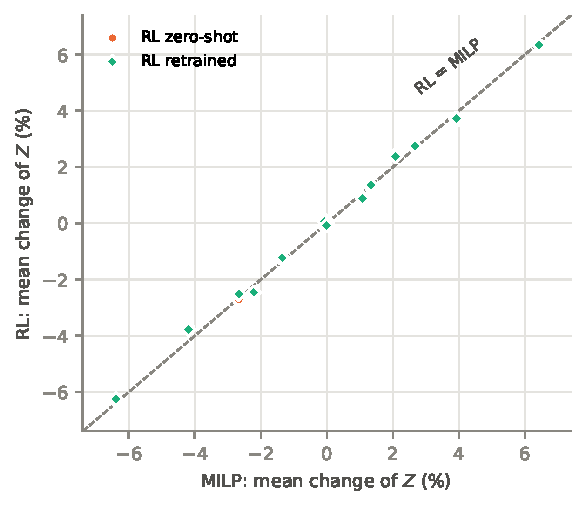
\includegraphics[width=0.56\textwidth]{figures/exp_agreement.pdf}
\caption{Mean $\Delta Z$ per variant: RL (zero-shot and retrained) against the MILP. Points on the diagonal mean
the two methods measure the same effect.}
\label{fig:agreement}
\end{figure}
The retrained RL agrees with the MILP to within \fagreeRtMean{} percentage points on average
(zero-shot \fagreeZsMean), and the sign agrees for all \fagreeSign{} of \fnVariants{} variants where the effect is
above noise. Because the two methods fail on \emph{different} instances (RL even places \frlOnlyFromNoPlan{} that
the MILP could not), their agreement on the \emph{effects} is not a shared bias --- it is confirmation.

\subsection{Theory, evidence and cause line up}
For every experiment the proposition's predicted direction, the measured number, and the practical mechanism point
the same way: E5 splits into an assignment lever and a level lever exactly as Proposition~\ref{prop:e5} says; E6's
size is read off the cost anatomy; E1, E2 and E8 obey the monotonicity/complementary-slackness arguments and the
direction check; E9 follows the charging-time law and E10 the affinity law, with the predicted asymmetry and
elasticity. When a derivation, two solvers and an operational story agree, the result is as well supported as this
kind of study allows.

\inshort{Every headline number is backed three ways: a direction the optimiser provably cannot break (0 violations
in 4\,000 optimal pairs), agreement of two independent methods (within \fagreeRtMean{} points), and a proposition
that predicts it.}

%=====================================================================
\section{Limitations}
\label{sec:limits}
\begin{itemize}
  \item \textbf{Placeholder sensitivities.} Apart from the segment share and the income distributions, the customer
  numbers are reasoned guesses; the experiments show \emph{how much} each matters, not its true value.
  \item \textbf{One change at a time.} Interactions (cheaper \emph{and} more vans, more demand \emph{and} more
  power) are not tested.
  \item \textbf{Time limit.} 223 of 560 baseline instances stop at 300\,s; effects smaller than the typical gap are
  read reliably only on the instances optimal in both (Table~\ref{tab:direction}).
  \item \textbf{Static demand.} All requests are known at time 0; real requests arrive during the day.
  \item \textbf{RL.} No optimality guarantee, one training run per model, and it under-uses vans, so the exact van
  policy is taken from the MILP. E9--E10 are RL-only (no MILP), justified by the close MILP--RL agreement on E1--E8.
  \item \textbf{Equity} is described (who queues, who pays, who feels what) but is not part of the objective.
\end{itemize}

%=====================================================================
\section{Conclusions}
\label{sec:concl}
\begin{enumerate}
  \item \textbf{Segment, not income, decides van use.} Vans are a service for rich \emph{private} owners; taxis
  take them only to escape a queue. This is rule \textbf{(T1)}--\textbf{(T3)} and it holds across every experiment.
  \item \textbf{The cost is driven by energy and by the poor.} Charging demand ($\pm22$\,\%) and station power
  ($\pm12$--20\,\%) are the largest levers because most of $Z$ scales with the energy charged; among the customer
  tastes, how a poor taxi driver feels money ($\pm6.4$\,\%) dominates, because taxis are the majority and the
  tariff is the biggest cost.
  \item \textbf{Price sets who gets vans; capacity sets who can be served.} The van tariff and the personal value
  of station time move the van share; the fleet size, the guns and the power decide feasibility --- below a point
  they strand cars rather than merely cost money.
  \item \textbf{The results are trustworthy.} Two independent methods agree to a fraction of a per cent, every
  provable direction holds with zero violations, and each number has a proof behind it.
  \item \textbf{Modelling guidance.} Van recharging can be dropped (E8). Effort to measure parameters should go
  first to the energy demand, the station power, and the commercial money sensitivity and downtime rate.
\end{enumerate}

\inshort{Formulation~4's one new fact --- personal versus commercial --- explains the whole plan: vans for rich
private owners, queues for taxis and the poor. Cost is governed by energy, power and the majority's money
sensitivity; feasibility by capacity. Every conclusion is backed by theory, by two agreeing methods, and by a
direction the optimiser cannot break.}

\vfill
{\footnotesize\emph{Reproducibility.} All figures, tables and numbers in this report are generated from the result
files by \code{report/make\_report\_f4.py} (which writes \code{figures/}, \code{tables/}, \code{numbers.tex});
the document is \code{report/analysis\_report\_f4.tex}. Every plan, from either method, is scored by the same
independent checker of constraints (2)--(23) and objective~\eqref{eq:obj}.}


\end{document}
